\documentclass[journal=langd5,manuscript=article]{achemso}
%\usepackage[margin=1in]{geometry}
\usepackage{rotating}
\usepackage[T1]{fontenc}
\usepackage[utf8]{inputenc}
\usepackage{flafter}
%\usepackage{floatflt}
\usepackage{placeins}
\usepackage{siunitx}
\usepackage{graphicx}
\graphicspath{{./figures/}}% Include figure files
%\usepackage{epstopdf}
\usepackage{dcolumn}% Align table columns on decimal point
\usepackage{appendix}
\usepackage{amsmath}
\usepackage{cases}
\usepackage{calc}
\usepackage{amssymb}
\usepackage[dvips]{color}
\usepackage{color}
\usepackage{enumitem}
\usepackage[final]{changes}
\usepackage{indentfirst}
\usepackage{hyphenat}
\usepackage{xspace}
\usepackage{subcaption}
\usepackage{booktabs}
\usepackage{multirow}
\usepackage{tabularx}
\usepackage{xcolor}
\usepackage[displaymath, mathlines]{lineno}
\usepackage{setspace}
\newcommand{\tbxmulticol}[3]
    {\multicolumn{#1}
                 {>{\centering\hsize=\dimexpr#1\hsize+#1\tabcolsep+\arrayrulewidth\relax}#2}
                 {#3}}
\newcommand{\ra}[1]{\renewcommand{\arraystretch}{#1}}
%\newcommand{\cmpersec}{$\frac{\text{cm}}{\text{s}}$~}
\newcommand{\cmpersec}{cm/s~}
\newcommand{\etal}{\textit{et al.}}
\newcommand{\na}{Na\textsuperscript{+}}
\newcommand{\cl}{Cl\textsuperscript{-}}
\newcommand{\PM}{$\pm$~}
\newcommand{\invnm}{$\text{\si{\nm}}^{-1}$~}
\newcommand{\nmeter}{\si{\nm}~}
\renewcommand{\arraystretch}{1.8}
\newcommand{\TODO}{\hl{TODO}~}
\newcommand{\about}{$\sim$}
\newcommand{\aangstroms}{{\aa}ngstr{\"o}ms}
\newcommand{\aangstrom}{{\aa}ngstr{\"o}m}
\newcommand{\sigmaij}{$\sigma_{ij}$}
\newcommand{\epsilonij}{$\epsilon_{ij}$}
\newcommand{\db}{$\text{D}_\text{B}$}
\newcommand{\dhh}{$\text{D}_\text{hh}$}
\newcommand{\dc}{$\text{2D}_\text{C}$}
\newcommand{\beginsupplemental}{%
    \setcounter{table}{0}
    \renewcommand{\thetable}{S\arabic{table}}%
    \setcounter{figure}{0}
    \renewcommand{\thefigure}{S\arabic{figure}}%
}
 \setlength {\marginparwidth }{2cm}

%\documentclass[10pt,preprint,times,3p]{elsarticle}
%\input{preamble}
%\newcommand*{\COMPLETE}{}%
%\bibliographystyle{elsarticle-num}



\author{Matthew Saunders} 
\email{mwsaunders@usf.edu}
\affiliation[University of South Florida]{Department of Cell biology, Microbiology and Molecular Biology,
      University of South Florida, Tampa, Florida 33620}
\author{Vered Wineman-Fisher}
\affiliation[University of South Florida]{Department of Cell biology, Microbiology and Molecular Biology,
  University of South Florida, Tampa, Florida 33620}
\author{Eric Jakobsson}
\affiliation[Center for Biophysics and
      Computational Biology, University of Illinois] {Department of
        Molecular and Integrative Physiology, Beckman Institute for
        Advanced Science and Technology, Department of Biochemistry,
        Center for Biophysics and Computational Biology, University of
        Illinois, Urbana, Illinois 61801}
\author{Sameer Varma}
\affiliation[Univerisity of South Florida]{Department of Cell biology, Microbiology and Molecular Biology,
University of South Florida, Tampa, Florida 33620}
\alsoaffiliation[University of South Florida]{Department of Physics, University of South Florida, Tampa,
         Florida 33620}
\author{Sagar A. Pandit} 
\email{pandit@usf.edu}
\affiliation[Univeristy of South Florida]{Department of Physics, University of South Florida, Tampa,
Florida 33620}


\abbreviations{???}
\keywords{???}

\date{\today}

\title{A high dimensional parameter search method to determine force field mixing terms in molecular simulations}

\begin{document}
\linenumbers
\begin{abstract}
%    \input{abstract}
Molecular dynamics (MD) force fields for lipids and ions are typically developed independently of one another. 
In simulations consisting of both lipids and ions, 
lipid-ion interaction energies are estimated using a predefined 
set of mixing rules for Lennard-Jones (LJ) interactions. 
This, however, does not guarantee their reliability. 
In fact, compared to the quantum mechanical reference data, 
Lorentz-Berthelot mixing 
rules substantially underestimate binding energies of \na~ ions with small 
molecule analogues of lipid headgroups, yielding errors on the order of 80 and 130 kJ/mol, 
respectively for methyl acetate and diethyl phosphate. Previously, errors 
associated with mixing force fields have been reduced using approaches like `NB-fix' 
in which LJ interactions are computed using explicit cross terms rather than 
those from mixing rules. Building on this idea, we derive explicit 
lipid-ion cross terms that also may implicitly include many-body 
cooperativity effects.
Additionally, to account for interdependency between cross terms, 
we optimize all cross terms simultaneously by 
performing high-dimensional searches using our ParOpt software. 
The cross terms we obtain reduce the 
errors due to mixing rules to below 10 kJ/mol. 
MD simulation of lipid bilayer conducted using these 
optimized cross terms resolve the structural discrepancies between our previous 
simulations and small-angle X-ray and neutron scattering experiments. 
These results demonstrate that simulations of lipid bilayers with ions that are 
accurate up to structural data from scattering experiments 
can be performed without explicit polarization terms. 
However, it is worth noting that such NB-fix cross terms are
not based on any physical principle; a polarizable lipid model would be more 
realistic, and is still desired. 
Our approach is generic and can be applied to 
improve accuracies of simulations employing mixed force fields.
\end{abstract}


\doublespacing
\listofchanges
\section{Introduction}

Cellular membranes function as highly dynamic interfaces with many diverse components, 
including lipids, peptides, carbohydrates, and charged species like ionic salts.
Studies of these complex systems often benefit from computational methods, 
particularly molecular dynamics (MD) simulations~\cite{berkowitz:2019}. 
In our previous MD simulation studies, we characterized the effects of various 
monovalent and divalent ions on model 1-palmitoyl-2-oleoyl-sn-glycero-phosphatidylcholine (POPC) 
bilayers~\cite{pandit:2008:simulationtextbook,kruczek:2017,kruczek:2019,saunders:2019}. 
We reported that ions modify POPC bilayer structure with significant
effects on area per lipid and bilayer thickness. Similar results were also reported in MD simulations by
others~\cite{Bockmann:2003,cordomi:2008,gurtovenko:2008,Cordomi:2009,jurkiewicz:2012}.
Experiments characterizing bilayer structures in the presence of ions
have not been as numerous as simulation studies. However, experimental findings indicate that 
dissolved salts at physiological concentrations do not modify bilayer structure
significantly~\cite{pabst:2007,petrache:2006:swelling,uhrikova:2008}.
Specifically, Petrache \etal~ performed small angle X-ray scattering (SAXS) experiments on
multilamellar vesicles of 1,2-dilauroyl-sn-glycero-3-sn-glycero-phosphatidylcholine 
as well as other lipids in KCl and BrCl salt solutions, 
and reported that while small changes can be seen in the
X-ray scattering form-factor due to the 
salts, 
the fitted electron density profiles are essentially identical for
systems with and without 
salt~\cite{petrache:2006:swelling}. 
Similarly, Pabst \etal~found no significant change in bilayer structure 
for POPC bilayers in NaCl salt at or below 1 M concentration~\cite{pabst:2007}.
Furthermore, Uhrikova \etal~reported small structural changes using small angle neutron scattering
(SANS) experiments on 1,2-dipalmitoyl-sn-glycero-3-sn-glycero-phosphatidylcholine 
vesicles interacting with CaCl$_{2}$~\cite{uhrikova:2008}. 
Taken together, these results point to a general discrepancy between structural data 
from MD simulations and scattering experiments.

The reliability of MD simulations depends greatly on the force field (FF) parameters 
used for describing intra- and inter-molecular interactions. 
While FF parameters of lipids, including ours, are developed with great accuracy and care, 
we note that they are derived in the absence of ions. 
Similarly, ion parameters are also derived in the absence of lipids~\cite{joung:2008}. 
When simulations of bilayers are conducted in salt solution, 
ion-lipid interactions are computed using FF mixing rules. 
In our previous MD simulations of POPC bilayers in salt solutions, 
we employed our gromos43A1-S3 lipid FF parameters~\cite{chiu:2009} 
that were developed for use with SPC/E water to determine lipid-lipid and lipid-water interactions. 
Ion-ion and ion-water interactions were described using Joung and Chetham~\cite{joung:2008} parameters, 
also developed for use with SPC/E water. 
Lipid-ion interactions were estimated using Lorentz-Berthelot (LB) 
mixing rules for Lennard-Jones (LJ) components
, and there was a significant change in bilayer 
structure compared to that of the bilayer without salt despite the relatively small initial salt concentration of 200 mM.
Does this suggest that the discrepancy between our MD predictions and experiments 
is the result of the LB mixing rules?  
Note that none of the MD simulations of lipid-ion interactions discussed above
include explicit terms to describe electronic polarization. 
Errors in mixing rules may, therefore, 
emerge if the high electric fields of ions induce 
cooperativity effects in lipid groups 
differently from those in water. 
Quantum mechanical (QM) studies, in fact, suggest that many-body 
cooperativty effects, such as polarization depend \deleted{strongly} 
strongly on ion-coordinator chemistry~\cite{varma:2010,wineman:2019}. 
It has also been postulated that these effects, and specifically 
electronic 
polarization may play an
important role in determining the structure and dynamics of lipid
bilayers
-- especially when interacting with 
ions~\cite{vacha:2010,vorobyov:2010,melcr:2018,chen:2021,lee:2008:origin}.

Small deviations from LB rules have been shown to have a significant
    effect on the behavior of systems of particles\cite{boda:2008:effects}, and
    it is possible that a systematic tuning of these parameters could be used to correct 
    for artifacts in a simulation~\cite{baker:2010:accurate,yoo:2012:improved,fyta:2012:ionic,mamatkulov:2013:force,venable:2013,
savelyev:2014:balancing,li:2015:representation,savelyev:2015:competition,jing:2017:study,reif:2017,wineman:2019}.
Such a `Non-Bonded-fix' (NB-fix) strategy has been shown to effectively improve 
protein-ion 
, protein-nucleotide, and ion-membrane interactions 
while retaining the commonly used form of the LJ 6-12 potential~
\cite{baker:2010:accurate,yoo:2012:improved,fyta:2012:ionic,mamatkulov:2013:force,venable:2013,
savelyev:2014:balancing,li:2015:representation,savelyev:2015:competition,jing:2017:study,reif:2017,wineman:2019}. 
Building on this idea, here we propose a more 
general approach to optimize interaction cross terms
for use with the 6-12 potential, 
and also validate its prediction in condensed phase simulations.  
We expand on the NB-fix method by
(a) optimizing all ion-lipid LJ cross terms simultaneously, and 
(b) implicitly including many-body cooperativity effects.
We consider simultaneous optimization of all cross terms to be critical, 
because of their strong, interdependent correlation with the target results~\cite{fogarty:2014:paropt}.
This high-dimensional optimization is performed using our software tool
ParOpt~\cite{fogarty:2014:paropt,fogarty:2014:thesis}.
Many-body cooperativity effects have been shown to be a major contributor to ion 
binding~\cite{varma:2010}
. Thus, it is important to include them in lipid bilayer simulations where ions are known
to coordinate simultaneously with multiple ligands~\cite{kruczek:2019}.

We show that the cross terms we obtain from this approach substantially improve 
ion-lipid interaction energies over those obtained from LB mixing rules. 
MD simulation of a POPC bilayer
 in 200~mM NaCl initial solution 
conducted using these optimized cross terms also 
resolves the structural discrepancies between our 
previous MD simulations and small-angle X-ray and neutron scattering experiments 
at low salt concentrations.


\section{Methods}

The method proposed here is generic and can be applied to any pair of
interacting species that use cross terms, and ensures that we are
reproducing macroscopic results based on the most accurate
representation of the local inter-molecular interactions.  We chose
small molecular analogues of the important ion binding
sites in the polar region of phospholipid
molecules. These molecules were also used as building block molecules in development of our lipid
FF~\cite{kruczek:2017,chiu:2009}. Specifically, we selected
methyl--acetate (MeAc) to represent the ester group binding the
acyl--chain to the glycerol backbone, and diethyl--phosphate (DePh) to
represent the headgroup phosphate and surrounding carbons (See insert on figure~\ref{fig:energies}). 
The overall goal was to take the substitution energy of ions from
water to the selected molecules, along with the corresponding
geometries, all computed using a benchmarked quantum mechanical framework, 
and optimize the interaction cross terms to reproduce these target data 
within the Molecular Mechanics force-field.

Combined analysis of results from experiments and \emph{ab initio} molecular dynamics simulations
in the aqueous phase suggest that~\na~ions prefer to directly coordinate 
with $\sim 5-6$ water molecules~
\cite{varma:2006:coordination,mason:2006:neutron,galib:2017:revisiting,timko:2010:dissociation,smirnov:2020}.
However, when coordinating with MeAc molecules, steric hindrance restricts the 
number of binding partners to fewer than four coordinating molecules.  
Thus, we limited the size of our MeAc clusters to up to four molecules around an ion. 
DePh has resonant oxygens on each molecule that potentially act as two binding sites, so we
limited these clusters to up to two molecules around a \na. These were
compared to the clusters of \na surrounded by up to four water
molecules.
In this work, we forgo modifying terms for \cl, as we have found in our previous work 
that anions do not bind to the bilayer headgroup significantly, and remain solvated 
by water molecules~\cite{kruczek:2017}.

\subsection{Quantum Mechanical Calculations}

Target data for our parameter optimization consisted of energies and geometries 
computed using a benchmarked density functional theory as implemented in  
the FHI-Aims software package~\cite{fhiaims}. 
Geometry optimizations were performed on the \na--(Water)$_{n}$,
\na--(MeAc)$_{n}, n\leq4$, and \na--(DePh)$_m, m\leq2$ clusters.
These clusters were first optimized using the MM force field used in 
Kruczek \etal and Saunders \etal~\cite{kruczek:2017,saunders:2019}. 
MM optimized structures were then further
optimized using the PBE0 functional~\cite{perdew:1996:generalized,adamo:1999:toward} 
with self-consistent vdW corrections~\cite{tkatchenko:2009}. 
We used the \emph{really tight} basis sets included in the FHI--aims software. 
This functional and basis set combination 
has been shown to perform well compared to
experiment and high-level quantum methods for many different chemistries of ion-ligand clusters~\cite{wineman:2019,wineman:2020:transferable,wineman:2020:improved}. 
Optimizations were performed with a force 
maxima of $10^{-3}$ $\text{eV}/\text{\AA}$~, with total energies converged
to within $10^{-6}$~eV. 
We computed substitution energies of these clusters as:
\begin{equation}
    \begin{split}
        E^{n}_\text{MeAc}&=E_{\text{\na--(MeAc)}_n}-nE_\text{MeAc}-E_{\text{\na--(Water)}_n}+nE_\text{Water}\\ 
        E^{n}_\text{DePh}&=E_{\text{\na--(DePh)}_n}-nE_\text{DePh}-E_{\text{\na--(Water)}_{2n}}+2nE_\text{Water}\text{,}
    \end{split}
    \label{eq:substitution}
\end{equation}
where $n$ is the number of solvent molecules
(see supplementary tables S1 and S2 for all of the QM
data used for this computation).  These substitution energies and
corresponding configurations were used as targets for the parameter
optimization.

\subsection{Parameter Optimization}

Parameter optimization is performed using our ParOpt software package~
\cite{fogarty:2014:paropt,fogarty:2014:thesis}.
This software is available for download at
\texttt{https://csmlabfs1.cas.usf.edu/Sites}.
We utilized the Nelder-Meade method to perform a search to simultaneously optimize 
all \sigmaij~and \epsilonij~ cross terms of \na~ions with MeAc and DePh molecules. 
Specifically, there are seven atom types in these two small molecules (table~\ref{tab:paropt}), and so we optimized
14 cross terms for the 6-12 LJ potential.
Error was
determined by comparing the optimized
geometries and substitution energies of each new parameter set to the
reference data from QM.  

Boundary constraints were imposed on \epsilonij~and \sigmaij~ to keep
the search space finite.  Table S3 in supporting information shows all of the
constraints placed on the parameter search. 
Additionally, we
constrained the NA--OM\* \sigmaij~ to be smaller than the \sigmaij~ for
NA--P to avoid unphysical conformations of DePh.  Boundary constraints are enforced 
by reassigning \sigmaij~or \epsilonij~ values that violate the bound to the boundary value. 
Throughout optimization we monitored constraint
violations and ensured that we did not select a final parameter set
that is the result of a constraint violation.  High--dimensional optimizations of
this nature may not have a unique solution; thus, we performed 200
independent optimizations with random initial parameter values. We
compared the parameter sets that best improved the substitution energy
without significantly compromising the conformational geometries.

Figure~\ref{fig:nmerror}a illustrates a representative
NM--trajectory that follows NM--error as a function of optimization step. In this case, the NM--error is
defined as an
equally--weighted combination of the mean absolute error of the
substitution energy and the distances between each atom in the cluster and the \na~ion. 
Each NM--move used is illustrated
as a point on the error curve 
(see Fogarty \etal~for complete description of NM algorithm and
moves~\cite{fogarty:2014:paropt}).
The insert shows the root-mean squared distance (RMSD) between the simplex vertices at each step. 
As is typical with the NM method, error drops exponentially during the
initial steps, and slows down towards the end of the optimization
process. The termination condition for the optimization run is the
collapse of the NM--simplex (defined by the RMSD~$\leq 10^{-10}$).
Figure~\ref{fig:nmerror}b shows all of the 291,870 \sigmaij-\epsilonij~ pairs tested 
between \na~ions and the non--carbon atoms in the 200 independent optimization runs,
and provides a visual perspective of the sampled parameter space.
The parameter set that yielded the lowest error, as discussed in the results section, was
chosen to perform MD simulations of a POPC bilayer.
%The resulting parameter set was used to perform a simulation of a lipid
%bilayer in NaCl salt solution in order to further characterize
%the changes introduced.

\subsection{Bilayer Construction}

We first constructed a monolayer of POPC lipids by placing 100 lipids on
a 10 nm by 10 nm grid, with excess space between the lipids to avoid overlaps in the lipid chains. 
Then we reflected this grid to create the second 
leaflet of the bilayer, resulting in a bilayer of 200 lipids. 

Assuming a conservative estimate of one binding site per lipid, we
need at least 200 \na~ ions in bulk solvent at the beginning of the simulation
to avoid complete depletion of bulk ions after equilibration. 
In order to do this we constructed a system with
double the size of the solvent block used in our previous
works~\cite{kruczek:2017,kruczek:2019}.  This larger system was
constructed by adding 60,000 waters to the system on a 3-D grid with
    excess space between waters, and randomly
replacing water molecules with 216 \na and 216 \cl. 
This results in an initial concentration of 200~mM, similar to our previous simulations.
This process resulted in a simulation box with dimensions $9.75  \text{~nm}\times9.75  \text{~nm}\times59.84 \text{~nm}$.

We energy-minimized the simulation box using the steepest descent
algorithm with a force tolerance of 50 $\text{kJ mol}^{-1}\text{nm}^{-1}$. 
Neighbor searching was performed every 2 steps. 
The PME algorithm was used for electrostatic interactions with a cut-off of 1.6~nm. 
A reciprocal grid with a spacing of 0.12~nm$^{-1}$ was used with 6th order B--spline interpolation. 
A single cut-off of 1.6~nm was used for van der Waals interactions.

We then performed a 200~ps constant pressure simulation at 290~K to
ensure the system was relaxed enough for further annealing. 
The box dimensions at the end of this were $7.86\text{~nm}\times7.86\text{~nm}\times32.90$\text{~nm}.
Annealing was started at 400~K, and the system was cooled to the production
simulation temperature of 300~K in steps of 10~K. 
Each step was simulated for 150~ps, giving a total annealing time of 1.5~ns. 
The annealing process shrunk the box dimensions to $7.97\text{~nm}\times7.97\text{~nm}\times32.14\text{~nm}$.
This final structure 
was used as the starting point for production run.

\subsection{Molecular dynamics}

All molecular dynamics simulations were performed with the GROMACS software package, 
version 5.1.6~\cite{abraham:2015,pall:2014,van:2005,lindahl:2001,berendsen:1995}.
We have utilized the SPC/E model for all waters~\cite{spce}. Lipid interaction
terms are described using the parameters in the gromos43A1-S3
parameter set developed by our group in previous work~\cite{chiu:2009}. 
The system temperature was held constant at the production run 
temperature of 300K using the Nos\`e--Hoover thermostat
with a coupling constant of 0.5~ps~\cite{nose:1983}. 
Pressure coupling was performed using the Parrinello-Rahman semiisotropic barostat,
which held the system pressure constant at 1 atm with a coupling
constant of 1.5~ps~\cite{parrinello:1981}. 
The P--LINCS algorithm was used to constrain all bonds in the system to allow for a 4~fs
integration timestep~\cite{lincs}. 
Integration was carried out using the Verlet scheme, 
with neighbor-list updates taken on every other integration step. 
We used a cutoff of 16~\AA for short--range electrostatics. 
Beyond this cutoff, we have used the smooth particle--mesh 
Ewald summation method to describe electrostatics~\cite{essmann:1995}. 
LJ interactions were calculated with a cutoff of 16~\AA. 
For all systems described, we have simulated continuously for 0.7~$\mu$s.

Simulated trajectories were analyzed using a combination of GROMACS
built--in analysis tools and in--house software developed on the
GROMACS API.

\section{Results and Discussion}

\subsection{Optimized Cross-Terms}

The final optimized parameters are detailed in table~\ref{tab:paropt}
alongside the original parameters computed using LB rules.  
We immediately note a general trend of an increase in the value of \epsilonij~ for the
non-carbon atom types. With our constraints on the carbon atoms, we have nudged the optimization
into gaining the binding energy by increasing the \epsilonij~ for the specifically electronegative atoms.
Values of \sigmaij~ have changed, but remained 
close to the original values in general, suggesting that the optimum 
distance to the minimum energy of the LJ potential is estimated well by LB rules. 
We can also see that no values of \sigmaij~ or \epsilonij~ violate the 
constraints described in table S3 in supporting information. 
We examined substitution energies and corresponding conformational geometries by running energy
minimization of the QM--optimized structures using the final parameter set. 
These were then analyzed using the GROMACS built--in energy and distance tools. 
The substitution energies and the conformations for
this parameter set are shown in figure~\ref{fig:energies} 
and in supplemental figure S1, respectively. 
We can see that for MeAc we have substantially improved substitution
energies relative to those obtained from using LB mixing rules, 
which started with an discrepancy of around 30--80~kJ/mol. We have also
improved the relative substitution between the clusters of various sizes. 
The substitution energies for DePh have also improved by a similar magnitude. 
The conformational geometries are largely unchanged, 
with a general trend of the binding distance to OM\* shrinking on the order of 0.25~\AA~in DePh. 
This shrinkage is common when optimizing both energies and conformations
with the relatively small number of free parameters corresponding to
the LJ cross terms~\cite{wineman:2019}.

We also note that the substitution energies for both molecule types improve more in the
larger cluster sizes. Larger clusters are more relevant to the dense
environment in the lipid headgroup region of the bilayer, 
as few, if any, ions bind to a single lipid at a time~\cite{kruczek:2017}. 
Furthermore, the substitution energy profile for MeAc has become much closer to that of the QM profile. 
Thus, these new parameters substantially improve the energetic balance
between the lipid--ion, lipid--water and ion--water interactions.

The conformational geometries were mostly unchanged with the new
parameter set, as even the original parameters do a good job in reproducing the QM--configurations. 
The least precise cluster appears to be for 4 MeAc, 
where the original LB parameters poorly represent the symmetries exhibited in the QM data. 
Even with the improvement from our new parameters, 
we may be missing behavior from explicit polarization effects that
cannot be captured properly by a non--polarizable model~\cite{varma:2010}.

\subsection{Validation of Parameters}

In order to characterize our new parameter set in a bilayer, 
we generated a 700~ns simulation of a bilayer of POPC lipids in NaCl salt solution, 
and we compared the results against a similar system that we simulated using
LB rules in our previous works~\cite{kruczek:2017,kruczek:2019}. 
These older trajectories for systems both with salt and without will be referred to, 
respectively, as  LB and `without salt.'  
We simulated our system with optimized cross terms, 
hence forth will be referred to as the `optimized' system, 
long enough to equilibrate the number of bound ions (see figure~\ref{fig:ioncoodcount}). 
We will further characterize this ion binding in a subsequent section.

\subsubsection{Bilayer Structure}

Bilayer structural parameters can be seen in table~\ref{tab:struc}.
The phospholipid component volumes $V_H$ and $V_C$ (lines 1 and 2) are
computed following the procedure outlined by Petrache \etal~\cite{petrache:1997}. 
The lipid chains are identified as starting at the first carbon attached to the lipid chain carbonyl oxygen, including the oxygen.
The atom groups not part of the lipid
chains are partitioned into the headgroup volume. 
We take the number--density of these component groups along with that of the solvent, 
and use them to optimize the objective function:
\begin{equation}
    \label{eq:volumeobj}
    \Omega(v_i)=\sum^{\rho_s}_{z_j}(1-\sum^{N_{\text{Groups}}}_{i=1}{(\rho_i(z_j)v_i)^2})\text{,}
\end{equation}
In the equation above, $\rho_i(z_j)$ is the number density of the $i$ component in the
$z_j$ slice of the box and $v_i$ is the corresponding component volume. 
The component volumes are then multiplied by the corresponding
number of particles per molecule per group -- 32 for the chain
particles, and 20 for the headgroup. 
This gives us the total volume per molecule for each group. 
The total lipid volume $V_L$ (line 3 in table~\ref{tab:struc}) 
is taken to be the sum of these two values. 
These remain relatively similar in all three systems, 
as this value is intrinsic to the lipid molecule 
and should not change with the inclusion of ions.

Structural data are obtained for lipid bilayers via small angle X-ray and neutron scattering
experiments as a one--dimensional form--factor. Data are then
fitted to a continuous function to retrieve number and electron
densities for the various lipid components~\cite{Nagle:2000,fogarty:2015}. 
Our simulations allow us direct access to the electron densities and number densities. 
The entries in table~\ref{tab:struc} are determined from these densities.

Figure~\ref{fig:eldens} shows the electron densities and corresponding bilayer form-factors. 
Form--factors are computed by taking the cosine--transform of the symmetrized electron densities.   
We note that the simulations carried out using LB rules produced a
thicker bilayer and had different details at the peak region of the density. 
The new parameter set results in similar electron density to that of the system without salt.
This is similar to the results reported by Petrache
\etal~ and Pabst \etal, where for systems with less than 1~M NaCl, 
the differences in the electron densities were not
discernible~\cite{petrache:2006:swelling,pabst:2007}. 
These electron densities are used directly to measure the value of \dhh, 
defined as the peak--to--peak distance (see table~\ref{tab:struc} line 4). 
The new parameter set corresponds to a smaller \dhh, similar to the system without salt.

In addition to \dhh, different measures are used to assess the bilayer thickness 
that relies on the probability densities of different components of the system.
It can be shown that \db~(see table~\ref{tab:struc} line 5) computed by integrating one minus
the probability density of solvent and ions is equivalent to the computation of the 
Luzzati thickness of the total bilayer~\cite{fogarty:2015,chiu:2009}.
We define probability of finding a particular component in a slice of the box as,
\begin{equation}
    \label{eq:probability}
    P_{i}(z) = \frac{\rho_i(z)}{\sum^n_{j}\rho_{j}(z)}\text{,}
\end{equation}
where $\rho_{i}(z)$ are the number densities for the 
component particles ($i$) of the system as a function of the 
z-position of each slice of the box, and the summation
ranges over all components in the particular slice.
Thus, 
\begin{equation}
\text{\db}=\int_{\text{Box length}}\big(1-P_{\text{water}+\text{ions}}(z)\big)\;dz\text{.}
\end{equation}
In table~\ref{tab:struc} line 2, the \db~is larger for the systems
with ions, but the value obtained using our new parameter set is closer to that of
the bilayer simulated without salt.

We use a similar definition of probability density for \dc, 
computed from the probability distribution of the lipid chains. 
This component is defined by the hydrocarbon chains starting after the ester--linkage
on both the Sn1 and Sn2 terminal of the lipid backbone. 
This value (line 6 in table~\ref{tab:struc}) is increased in the system simulated
with LB rules over the system without salt, 
as we reported in our previous work. 
However, the new parameter set yields a value similar to the system without salt, 
which is consistent with the smaller overall thickness of the bilayer 
simulated with optimized cross terms.

The differences in bilayer thickness are closely related to the
packing of the lipid chains in the hydrophobic core of the bilayer. 
When the chains become more disordered, 
the bilayer thickness typically drops~\cite{Nagle:2000}. 
Lipid chain ordering can be determined experimentally by performing NMR 
on specifically deuterated hydrocarbon chains. 
Since we lack hydrogen on our coarse--grained lipid chains, 
we cannot directly access the C--D ordering. 
Instead, we compute the chain order tensor $S_{\alpha\beta}$ defined as
\begin{equation}
    S_{\alpha\beta}=\frac{1}{2}\big\langle
    3\cos{\theta_\alpha}\cdot\cos{\theta_\beta}-\delta_{\alpha\beta}\big\rangle,
    \nonumber
\end{equation}
where the angles $\theta_\alpha$ and $\theta_\beta$ are the angles between the molecular
axis and the box z-direction. 
We then use this tensor to calculate the $S_{CD}$ as
\begin{equation}
    -S_{CD}^{\text{Saturated}}=\frac{2}{3}S_{xx}+\frac{1}{3}S_{yy}
\end{equation}
for saturated carbons~\cite{egberts:1988}, and as
\begin{equation}
-S_{CD}^{\text{Unsaturated}}=\frac{1}{4}S_{zz}+\frac{3}{4}S_{yy}\mp \frac{\sqrt{3}}{2}S_{yz}
\end{equation}
for unsaturated carbons~\cite{Douliez:1995}.  
These values are plotted per each carbon in the lipid chain in figure S2 in supporting
information.
As reported in our previous simulations, 
the addition of salt has an ordering effect on the lipid chains. 
This effect is also seen in our new parameter set; however, the ordering is less pronounced, 
which is consistent with the notion that the bilayer structure is not significantly altered 
at physiological salt concentration~\cite{pabst:2007,petrache:2006:swelling}.

While this result indicates a structure more consistent with experimental results, 
the detailed structure of a lipid bilayer is a result of the
delicate balance between ion--lipid, lipid--water, and ion--water interactions.
In order to fully understand how our new parameter set has altered the
overall bilayer structure, we next characterize the specific interactions
between these moieties.

\subsection{Membrane-Salt Interactions}

Both ions and solvent compete for the binding sites on the lipid headgroup. 
As seen in figure~\ref{fig:energies}, the new cross terms
produce a relatively stronger interaction between \na and lipid
headgroup components compared to that of the LB rules. 
Thus, there is potentially a reduction in the available binding sites for the solvent. 
To examine how the new cross terms have altered ion interactions with lipids in the bilayer, 
we first characterize the dynamics of ion binding to the lipid bilayer.

We define ion binding to the lipid bilayer when half or fewer
of its first shell coordinators are not waters. 
In order to compute the equilibrium binding constant, 
we must determine the equilibrium number of bound ions to the lipid surface. 
Figure~\ref{fig:ioncoodcount} shows the number of bound ions as a
function of time over the entire duration of the simulation. 
We note that even after 700~ns of simulation time, the number of bound ions
are not fully equilibrated. 
Thus, we use first--order reaction kinetics to
estimate the asymptotic number of bound ions.  
The first--order reaction kinetics are modeled as a differential equation:
\begin{equation}
    \frac{dN_b}{dt}=K_a \left(N-N_b\right)- K_d N_b,
\end{equation}
where $N_b$ are the number of bound ions, and $K_a,K_d$ are the association and dissociation
time constants, respectively.
The solution of this differential equation is:
\begin{equation}
    N_b(t)= \frac{K_{a}}{K_{a}+K_{d}} N
    \left(1-\exp\left[-\left(K_{a}+K_{d}\right)\left(t-t_0\right)\right]\right).
    \label{eq:ioncoodnumfit}
\end{equation}
This solution is fit to the data in figure~\ref{fig:ioncoodcount}, 
and the resulting fit is also plotted. 
The fitting parameters are listed in table~\ref{tab:struc}.
The first--order reaction kinetic model fits reasonably well to the 
data from both the systems, except in the beginning of
the simulation where the effect of the annealing process is more pronounced; 
however, we are only interested in the asymptotic
behavior of the fit as this is representative of the equilibrium state of the system. 
The asymptotic number of bound ions as $t\to\infty$, $A=\frac{K_{a}}{K_{a}+K_{d}} N$ 
(table~\ref{tab:struc} row 9), is larger in the system simulated with optimized terms.
We also report the timescale of ion binding $\tau=\frac{1}{\left(K_{a}+K_{d}\right)}$
for both systems (table~\ref{tab:struc} row 10). 
The timescale of binding in the system using optimized  cross terms is longer, 
and suggests that this system would need more time to equilibrate than the system simulated with LB rules.
Finally, we report the value of $\frac{K_a}{K_d}$ 
(table~\ref{tab:struc} row 11), which
we observe is much smaller with the new parameter set than compared to that
of the system simulated with LB rules.

To examine how specific interactions between ions and lipids are modified by the new parameters, 
we tracked the binding partners of ions across the box over the last 150~ns of simulation time. 
Moieties are considered to be bound to an ion if they are within a distance of 3.3 \AA~from the \na~ion. 
Several electronegative groups in the simulation can potentially bind to the \na~ion. 
We compute the number of these potential binding partners within the first shell of each \na~ion
across the simulation box. 
Ions are then sorted according to their box z-positions, and then the data are averaged over the last 150~ns. 
This is plotted in figure~\ref{fig:cood}. 
We note first that the total number of solvating oxygens of ions within the bilayer headgroup
region with the optimized parameter set has dropped by $\sim 1$ when
compared to ions in similar locations in the system simulated using LB rules. 
This is not surprising, given the dependence of ion coordination
preferences on the local environment~\cite{varma:2008:JACS}. 
The binding to other lipid oxygens has not been altered much by the new parameter set; 
however, we do note that water within the headgroup region does not appear to be strongly associated with ions. 

\subsection{Water Structure and Dynamics}

To further characterize the dehydration of ions in the new simulated system, 
we look to the lipid-- and ion--water interactions.
Figure~\ref{fig:waterdens} shows the number density of water as a
function of distance from the bilayer center for each of our simulated
systems, with the \dc~and \db~illustrated as dotted lines.  
We see that our new parameter set produces a bilayer
interface that has more solvent inside the headgroup region, 
between $10-25$~\AA~from the bilayer center. 
This density is more similar to that of the system simulated without salt. 
This suggests that the dehydration of ions in the system simulated with optimized parameters
does not correspond to a dehydration of the lipid bilayer.

Next, we characterize the orientational structure of the water.
Figure~\ref{fig:waterorder} examines the water order parameter across the simulation box. 
We identify perturbed water structure by examining first ($P_1$) and second ($P_2$) 
orientational order parameters for the
OW$\rightarrow$HW1 bond of water with respect to the z-axis of the simulation box ($\beta$). 
These order parameters are defined using the first and second 
Legendre polynomials with respect to the angle $\beta$,
\begin{equation}
    \begin{split}
    P_1&=\langle \cos\left(\beta\right) \rangle
    \\ P_2&=\frac{1}{2}\bigg\langle\left(3\cos^2\left(\beta\right)-2\right)\bigg\rangle
    \text{,} 
\end{split}
\end{equation}
where average is over all the waters in a particular volume slice of the box 
and then over simulation time.  
We plot these values as a function of distance from the bilayer center. 
$P_1$ denotes dipolar ordering of the bond vector and the bilayer normal direction, 
with a positive value indicating an average outward orientation 
and a zero value corresponding to an average perpendicular orientation to the
bilayer normal or a uniformly random orientation. 
We observe a similar pattern of ordering across the box in all systems; 
however, we see an overall reduction in ordering with our new parameter set when
compared to both the LB and the no--salt system. 
We also see the inner minimum of the order parameter moved further into the bilayer
when compared to LB, 
which is consistent with the larger quantity of water 
in this region that we observe in the water densities.

Following the protocol established in our previous work~\cite{saunders:2019}, 
we identify three regions within the bilayer interface, $B_{-1}, B_{+}, B_{-2}$. 
The $B_{-1}$ region is defined as the region of negative ordering starting at the bilayer center, and ending 
    when the order parameter values cross zero at the start of the $B_{+}$ 
    region. The $B_{+}$ region starts at the end of the $B_{-1}$ region, and 
    is the area of positive ordering, ending where the order parameter crosses
    zero again. The $B_{-2}$ region starts at the end of the $B_{+}$, and extends out to where the 
    second order parameter goes to zero. This was found by fitting an exponential function to this region 
    and taking the \replaced{scale parameter}{timescale} from that fit as the boundary with bulk solvent.
We find that water is significantly less perturbed by the bilayer with our new parameter set.  
We have also computed $P_2\cdot\rho_{\text{Water}}$, shown in shown in figure~\ref{fig:waterorder}(c). 
This value relates the amount of water in each region of the box and 
the overall ordering in the region. 
We still see significantly less ordering with the new parameter set, 
and even with the larger number of waters in the bilayer headgroup. 
The integral of this curve is related to the quadrupole splitting $\Delta \nu$ observed in
in deuterium NMR experiments~\cite{aaman:2003,kruczek:2017}.

This suggests that while there is more solvent in the interface, it is perhaps not
associated with either \na or lipids, and may remain less structured than
in the system simulated with LB rules.  
This can be further ascertained by the lateral diffusion coefficients of waters 
in each of the regions defined by $P_2$. 
We compute the mean square displacement (MSD) for water oxygens
in each region by first tracking which waters remain in the region. 
Any waters that leave the region are removed from the MSD calculation. 
We chose a duration of 100~ps to track the MSD in order
to have a sufficiently long time for the MSD to become linear, 
while still maintaining a statistically significant number of waters in the slice. 
A line is fit to the middle 80\% of the MSD, and the fitted
slope is used to calculate the diffusion coefficient following
Einstiein's relation for 2D diffusion
\begin{equation}
\lim_{t \to \infty}\frac{\big\langle (r(t) - r(0))^2 \big\rangle}{(t-t_0)} = 4D. 
\end{equation}
These values can be seen in table~\ref{tab:diff}. 
We note that the water in the headgroup region, corresponding to $B_{-1}$ and $B_+$, 
diffuses slightly faster with the new parameter set, 
indicating more mobile water in these regions. 
However, the computed diffusion coefficients are within the error bars that of the system simulated with LB rules. 
Diffusion in the $B_{-2}$ and $Bulk$ regions are similar in both systems, 
as these are mostly outside of the bilayer and should not be affected by the new parameter set.


\subsection{Bilayer Electrostatics}

We further characterize the electrostatic properties of our bilayer
systems by computing the electrostatic potential across the simulation box. 
We do this following the protocol used in Saunders \etal
~\cite{saunders:2019}. We first compute the charge density of the
system components. We integrate this distribution twice, setting both
constants of integration to be zero to enforce a zero value for the
electric field in bulk solvent and a zero electrostatic potential at
the box edge. This is accomplished by taking the average value of the
electric field in the \emph{bulk} region of the box defined earlier,
and subtracting this value from all points. Due to the larger system
size in the optimized system, we needed to compute the average value of a much
larger region than in LB in order to apply boundary conditions. We
then integrate again to get the electrostatic potential. This result
can be seen in figure S3 in supporting information. The shape of the potential
is largely unaltered within fluctuations. Systems simulated with the
optimized parameters and with LB rules both have a similar bilayer dipole potential, 
which remains elevated over
the system without salt, by $\sim$ 220~mV.  We report 
that the optimized system has a slightly
elevated bilayer dipole potential compared to the system simulated with
LB rules, increased by $\sim$ 12~mV.
This may be a direct result of the larger number of
ions bound to the bilayer in this system.  We also note the system simulated with optimized cross terms
has different details
throughout the electrostatic potential compared to the system simulated with LB rules and in the
system without salt, however these are within fluctuations and cannot be used to draw conclusions.

Poisson--Boltzmann (PB) theory is a mean field approximation for
solvated ions near an interface. Experimentally PB theory is used to
assess the surface potential of the lipid bilayers. We also examine
the behavior of the ions in bulk solvent under the framework of PB
theory. Following the procedure used in our previous
work~\cite{saunders:2019}, we fit the number density of \cl ions in
the solvent--occupied region of the box to a Poisson-Boltzmann
distribution, using the inverse Debye length $K$ and the density of
\cl at the center of the solvent occupied region of the box $\rho_0$
as fit parameters. 
The density is modeled as:
\begin{equation}
    \label{eq:gcdens}
    \rho (z)= \rho _{0} \exp{(- \bar{z} e \beta \psi (z))},
\end{equation}
where $\rho_0$ is the number density of the ion at the center of the
solvent--occupied region of the box, $\bar{z}=1$ is the valency of the
ion in the system, $\beta=\frac{1}{k_b T}$, $e$ is the charge on an
electron, and $\psi(z)$ is the electrostatic potential. We then assume
the form of $\psi(z)$ to be the sum of two Debye-Huckel
potentials~\cite{israelachvili:2011:intermol} reflected across the
center of the solvent--occupied region of the box:
\begin{equation}
    \begin{split}
    \psi_1(z)&=\psi_s \exp(-K(z+\frac{D}{2})) \\
    \psi_2(z)&=\psi_s \exp(K(z+\frac{D}{2})) \\
    \psi(z)&=\psi_1 + \psi_2\text{,}
    \label{eq:gcpot}
\end{split}
\end{equation}
where $D$ is the distance from the hydration boundary of one bilayer leaflet
to the next across the solvent, $K$ is the inverse Debye length, and $\psi_s$ is the surface potential:
\begin{equation}
    \psi_s = \frac{\varsigma}{\varepsilon_0\varepsilon K}\text{.}
\label{eq:gcspot}
\end{equation}
%, given by
%\begin{equation}
%K=\sqrt{\sum_i{\rho_{0,i}\bar{z^2_i}\frac{e^2}{\epsilon_0 \epsilon k_bT}}}
%\label{eq:gcK}
%\end{equation}
\deleted{We used a value of $D=13.167$ nm for the LB system, and $D=27.01$ nm for the system simulated with optimized parameters. }
\added{The LB system yielded a value of $D=13.167$ nm and the system }
\added{simulated with optimized parameters, containing twice as many }
\added{solvent molecules, }
\added{gave a value of $D=27.01$ nm.}
We take the surface charge density $\varsigma$ from the charge density inside
of the hydration boundary of the lipid bilayer. Since only ions
contribute a net charge to our system, we compute this using only the
charge density of ions in the system. 
This value was computed to be $\varsigma=0.13$ \emph{e} nm$^{-2}$ for the system simulated with LB rules, and 
$\varsigma=0.11$ \emph{e} nm$^{-2}$ for the system simulated with the new parameters.
Our fitting procedure yielded 
number densities $\rho _{0}=0.043\text{nm}^{-3}$ for the system simulated with LB rules, 
and $\rho _{0}=0.079\text{nm}^{-3}$ for the system simulated with optimized parameters.
The fitted inverse screening lengths were found to be $K=0.91 \pm 0.014$ nm$^{-1}$ for the LB rules simulation 
and $0.94 \pm 0.018$ nm$^{-1}$ for the system simulated with optimized parameters.
The resulting fit and predicted
density of \na ions and electrostatic potential can be seen in
figure~S4 in supporting information. 
We see the results from our simulation
represented by points with error bars, while PB theory results are
shown in solid lines.  We see excellent agreement in the \na density
profile away from the bilayer surface, and reasonable agreement in the
electrostatic potential. From this we can see that the optimized and LB
systems both exhibit similar ionic distributions with models used to
describe electrophoretic mobility
experiments~\cite{israelachvili:2011:intermol}.

\section{Conclusions}

Mixing rules are often relied upon to compute non--bonded cross terms 
for interacting molecules in molecular simulations. 
However, when mixing force--fields that have been developed independently of each other, 
inaccuracies may develop. 
Here we demonstrate one such case and propose a rigorous solution. 
MD simulations conducted using predefined mixing rules for 
non-polarizable force fields developed separately for ions and lipids 
have always produced very pronounced salt-induced structural changes in lipid bilayers. 
Contrary to this, most experimental observations point to a 
moderate or even an insignificant change in bilayer structure at physiological salt concentrations. 
We resolve this discrepancy by explicitly parameterizing ion--lipid cross terms
using our procedure {\em ``Many Body Non Bonded fix''} (MB-NB-fix). 
It is based on the NB-fix method employed in previous works
~\cite{baker:2010:accurate,yoo:2012:improved,fyta:2012:ionic,mamatkulov:2013:force,venable:2013,savelyev:2014:balancing,li:2015:representation,savelyev:2015:competition,jing:2017:study}
and utilizes ParOpt software developed in our lab~\cite{fogarty:2014:paropt}\cite{fogarty:2014:thesis}.
We note that after applying the optimized parameters for \na--lipid interactions, the 
bilayer structure conforms more to experimental
observations while all other properties such as solvent structure,
electrostatic potential, and dynamic properties are approximately
similar to that obtained with those obtained with LB parameters. 
We note that we have not applied this method to optimize \cl~ interactions terms, which
may still further affect the bilayer structure. This will be the subject of future work.

The MB-NB-fix method proposed here is a 
general method which can be used to derive mixing
terms for simulations with independently developed force fields. 
This method will be used in future work to improve other sets of mixed force-fields, including 
those of other monovalent ions and the gromos 43A1-S3 lipids, and between these lipids and amino-acids for use in proteins.
Furthermore, many body cooperativity effects, such as ion-induced polarization 
in lipid molecules may be critical to further improving
the reproduction of lipid bilayer structure.
A correct approach to incorporate these effects to our simulation 
would be to have explicit polarization terms in 
our simulation models. This is complicated, as most existing polarizable 
simulation models are either not very effective
at accurately reproducing polarization effects or are
much more computationally expensive compared
to classical non-polarizable simulations. The MB-NB-fix method
has potential to become an ideal solution for mixing force-fields, including
polarizable and non-polarizable models in the same system 
to construct simulations that are tractable yet accurate.

\section{Supporting Information}
Table S1 and S2 contain raw data from QM calculations described in the methods section. Figure S1 shows
the geometry of optimized structures from QM calculations compared to those computed with LB rules and those
computed with the optimized parameter set. Table S3 contains the constraints applied to the Nelder–Meade constraints
applied to the parameter search. Figure S2 contains a comparison of lipid chain deuterium order parameters between
the simulated systems. Figure S3 is the electrostatic potential as a function of distance from bilayer center.
Figure S4 demonstrates Poisson-Boltzmann theory predictions and simulation results.
\section{Acknowledgements}
Computing support was sponsored in part by NSF MRI CHE-1531590,
CNS-1513126 and IIS-1253980. Authors MS, VWF, and SV acknowledge support
provided NIH under the grant number R01GM118697.

\bibliography{refs}
\newpage

\section{Table and Figure Captions}

Table \ref{tab:paropt}: Force--field cross terms. Original terms, as used in the system simulated with LB rules were computed by applying Lorentz-Berthelot mixing rules to the LJ parameters of \na and each lipid component atom type. Optimized parameters are the result of the NM--optimization using ParOpt~\cite{fogarty:2014:paropt,fogarty:2014:thesis}. All constraints
on the search space can be seen in figure S3 in supporting information.
\\\\
Table \ref{tab:struc}: Bilayer structural parameters. \dhh~is the peak--to--peak distance from the electron density of the
        lipid bilayer, and is a measure of bilayer thickness. Bilayer thickness \db~and chain thickness \dc~are computed from
        number densities of the solvent and the lipid chains, respectively. $V_H$, and $V_C$ are the volumes of the headgroup and lipid chains computed
        using the method from Petrache \etal~\cite{petrache:1997}. $V_L$ is the sum of $V_H$ and $V_C$. 
        Rows 7-11 contain kinetic parameters for ion binding to membrane. These parameters come from fitting 
        the equation $ N_b(t)= \frac{K_{a}}{K_{a}+K_{d}} 
            N\left(1-\exp\left[-\left(K_{a}+K_{d}\right)\left(t-t_0\right)\right]\right)$ to the data for the number of ions
            bound to the lipid bilayer across the simulation time. 
            $A$ is the asymptotic number of ions bound to the lipid bilayer, and can be used as the expected number of ions
        that will bind to the system at equilibrium. $\tau$ is the characteristic timescale of the fitted function. $n_0$ is the number of ions bound at the beginning
        of the production run of the simulation. $K_D$ and $K_A$ are the computed binding association and dissociation constants, and $K_A/K_D$ is the binding
    rate constant.
\\\\
\\\\
Table \ref{tab:diff}: Diffusion coefficients of water in different regions of the lipid bilayer, 
defined by the shape of the second orientational order parameter of water molecules in the box. 
These regions are defined by the shape of the distribution of the second 
    orientational order parameter across the simulation box. $B_{-1}$ is the region 
    of negative ordering starting at the bilayer center, and ending 
    when the order parameter values cross zero. 
    $B_{+}$ starts at the end of the $B_{-1}$, and is the region of positive ordering ending where the order parameter 
    becomes negative. This starts the $B_{-2}$ of negative ordering, extending out to where the 
second order parameter goes to zero, where we have $Bulk$ solvent.
We see that the optimized parameters result in slightly 
    increased diffusion in the solvent, which correlates with the reduced
    ordering of the water dipoles and quadrupoles in the
system.\\\
%Table \ref{tab:gctheory}: Poisson-Boltzmann theory parameters. 
%\\\\


\clearpage

Figure \ref{fig:energies}: Substitution energies for \na~clusters computed as described
in equation~\ref{eq:substitution}. 
In black we see the energies of systems computed using the standard 
mixing rules, in red we have the energies from benchmarked DFT, 
and in blue the optimized results. 
We see a significant
error with the standard LB mixing rules, which is substantially improved with our new optimized cross terms. 
The insert shows an diagram of POPC, and
the small molecules Methyl-Acetate (MeAc) and Diethyl-Phosphate (DePh) 
that were used to represent the major \na~interaction sites on the POPC molecule.
\\\\
Figure \ref{fig:nmerror}: (a) Representative Nelder--Meade (NM) optimization run. Each point
    represents a move that the NM simplex can make while navigating the parameter space 
    (See Fogarty \etal~for a full description of the
    Nelder--Meade algorithm and available moves~\cite{fogarty:2014:paropt}). The insert illustrates the 
    RMSD between the simplex vertices.
    The optimization is considered converged when the simplex collapses, which is defined by an RMSD~$\leq 10^{-10}$.
    (b) Map of all \sigmaij~ and \epsilonij~ tested for interactions of \na~with non--carbon atom types 
    in the 200 optimizations performed to find our final optimized set of cross terms. A total of
    291,870 combinations of parameters were tested, shown color-coded according to their NM error.
\\\\
Figure \ref{fig:ioncoodcount}: Number of ions bound to the lipid bilayer as a function of simulation time. 
The exponential fits to this data are also shown. These fits are used to compute the asymptotic
number of ions bound as well as binding rate constants.
`Total' refers to the total number of ions in each simulation box.
A membrane bound ion is defined as having half or fewer of its first coordination shell
occupied by water molecules.  
\\\\
Figure \ref{fig:eldens}: Electron densities of the simulated bilayers (a), and corresponding bilayer form--factors (b).
        Electron densities as obtained using the GROMACS density tool,
    centered at the minimum to define the bilayer center, and with the electron density of solvent subtracted.
    The simulated with optimized parameters appears to lack the large peak seen in the system simulated
    with LB rules, and appears more similar to the
bilayer structure of a bilayer simulated without salt. 
This is further reflected in the bilayer form--factor, 
computed by taking the cosine--transform of electron density. Experimental
SAXS results are for a POPC bilayer in pure solvent~\cite{fogarty:2015}. We see the first lobe
of the optimized system moves closer to the experimental results and the form--factor of a system without salt. This lines up with experimental results, that have shown small, if any, change
in the bilayer SAXS form--factor~\cite{pabst:2007,petrache:2006:swelling,uhrikova:2008}.
\\\\
Figure \ref{fig:cood}: Chemistry of \na~inner shell coordination as a function of distance from bilayer
center. Compared to the system simulated with LB rules (a), the system simulated with optimized cross terms (b)
        yields a lower \na~total coordination number within the headgroup region of the bilayer. 
        This drop in coordination appears to be due to a greater dehydration of the ions in this system.
\\\\
 Figure \ref{fig:waterdens}: Water density at the bilayer interface. We illustrate the regions regions $B_{-1}$, $B_+$, $B_{-2}$ and $Bulk$ for each system with dotted lines.
    We see that the optimized cross terms yield a greater density 
    of solvent in the $B_{+}$ and $B_{-1}$ regions over the system simulated with LB rules. 
We also see the density in these regions of the system optimized
with optimized cross terms is more similar to that of the system without salt.
\\\\
Figure \ref{fig:waterorder}:
Water orientational order parameters $P_1$ (a) and $P_2$ (b), 
and the product of the water number density and $P_2$ (c). We see in $P_1$ and $P_2$ less
    ordering in the waters in the optimized system, suggesting that waters may be less strongly interacting with ions or lipid components. We denote the four regions of the lipid bilayer based on the shape of the $P_2$ data as dotted lines
    in (b)~\cite{saunders:2019}. We have not included these regions
 for the system without salt, as the $P_2$ data does not include the same details as the systems with salt. The integral of (c) is related to the
 quadrupolar splitting constant $\Delta \nu$ found in deuterium NMR experiments. This also gives a closer look at how solvent is ordered in the headgroup while
 accounting for the amount of solvent in the region. We see that optimized cross terms result in a significant drop in the area under the curve, which is much closer
 to the shape of the data from the system without salt. 
 The regions $B_{-2}$ and $Bulk$ are not within the bilayer
 headgroup, and are expected to be less affected by the new parameter set.
\\\\
\clearpage

\section{Tables and Figures}
\begin{table}
    \caption{ }
    \label{tab:paropt}
    {\footnotesize
    \begin{tabularx}{\textwidth}{X|X|X|X|X|}
              &\tbxmulticol{2}{X|}{Original}&\tbxmulticol{2}{X|}{Optimized}\\\hline
              &\sigmaij (nm) &\epsilonij (kJ/mol) &\sigmaij (nm) &\epsilonij (kJ/mol)\\\hline
        NA-CH3&0.295&1.100&0.235&0.700\\
        NA-CH2&0.312&0.772&0.237&0.809\\
        NA-OA &0.256&1.120&0.211&3.035\\
        NA-P  &0.277&1.900&0.301&0.483\\
        NA-OM*&0.252&1.221&0.211&1.445\\
        NA-CO*&0.335&0.362&0.315&0.758\\
        NA-O* &0.251&1.221&0.216&2.440\\
              \end{tabularx}
          }
\end{table}
\clearpage
\begin{table}
    \caption{ }
    \label{tab:struc}
    {\footnotesize
    \begin{tabularx}{\textwidth}{X|X|X|X}
         &Without salt      &LB                 &Optimized\\\hline
        $D_{HH}$~(\AA)&37.44 $\pm$ 1.07  &40.18 $\pm$ 1.04   &37.64 $\pm$ 0.88 \\
        $D_B$~(\AA)   &36.54 $\pm$ 0.47  &40.90 $\pm$ 0.31   &39.36 $\pm$ 0.43\\
        $2D_C$~(\AA)  &27.07 $\pm$ 0.34  &30.33 $\pm$ 0.29   &28.97 $\pm$ 0.34     \\
        $V_H$~(\AA$^3$) &310.68 $\pm$ 1.14 &316.13 $\pm$ 0.83  &314.81 $\pm$ 0.75          \\
        $V_C$~(\AA$^3$) &904.89 $\pm$ 1.28 &891.79 $\pm$ 1.65  &896.50 $\pm$ 1.19         \\
        $V_L$~(\AA$^3$) &1215.57 $\pm$ 1.00&1207.92 $\pm$ 1.57 &1211.32 $\pm$ 1.21    \\
        $K_{A}$ (ns$^{-1}$)        &N/A & $7.12\times10^{-3}\pm8.18\times10^{-5}$     &$2.65\times10^{-3}\pm1.74\times10^{-5}$ \\
        $K_{D}$ (ns$^{-1}$)        &N/A & $3.20\times10^{-3}\pm4.75\times10^{-5}$     &$3.58\times10^{-3}\pm2.83\times10^{-5}$ \\
        $A$                        &N/A & $74.51$                        &$91.88$ \\
        $\tau$      (ns)           &N/A & $96.73$                      &$160.54$ \\
        $K_{A}/K_{D}$              &N/A & $2.225$                           &$0.74$ \\
              \end{tabularx}
          }
\end{table}
\clearpage
\begin{table}
    \caption{ }
    \label{tab:diff}
    {\footnotesize
    \begin{tabularx}{\textwidth}{X|X|X|}
              &LB ($\times 10^{-10} m^2/s$)&Optimized ($\times 10^{-10} m^2/s$)\\\hline
        $B_{-1}$ &1.11 $\pm$ 1.10& 1.88 $\pm$ 2.41   \\
        $B_+$    &4.23 $\pm$ 1.14& 6.11 $\pm$ 2.83  \\
        $B_{-2}$ &18.11 $\pm$ 4.23&21.29 $\pm$ 4.12 \\
        $Bulk$   &27.32 $\pm$ 1.15 &27.25 $\pm$ 1.36 \\
              \end{tabularx}
          }
\end{table}
\clearpage


\begin{figure}[htb]
    \caption{ }
    \label{fig:energies}
    %\includegraphics[width=\textwidth,trim=-3cm 0 0 0]{energies_combined_final.eps}
    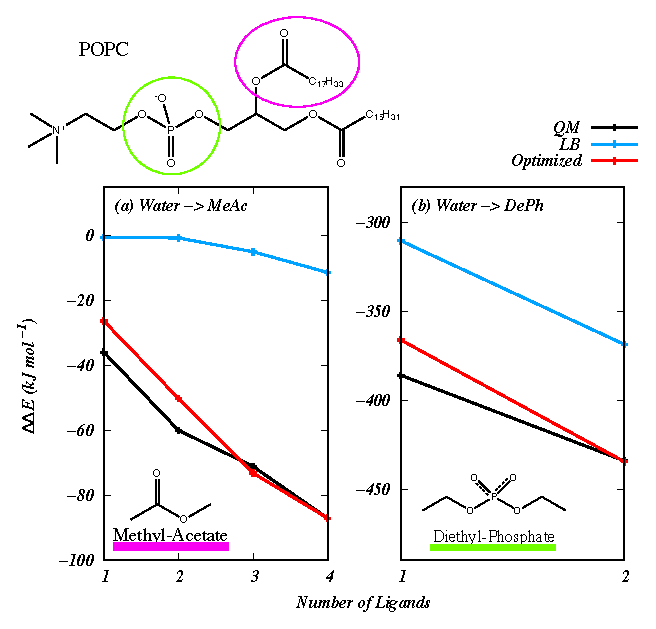
\includegraphics[width=\textwidth,trim=-3cm 0 0 0]{figure_1.eps}
    %MOLECULE ON THE SIDE
\end{figure}
\clearpage
\begin{figure}[htb]
    \caption{ }
    \label{fig:nmerror}
    %\includegraphics[width=\textwidth,trim=-3cm 0 0 -3cm]{7_NA_RERUN_CCONSTRAINED_EQ_3.eps}
    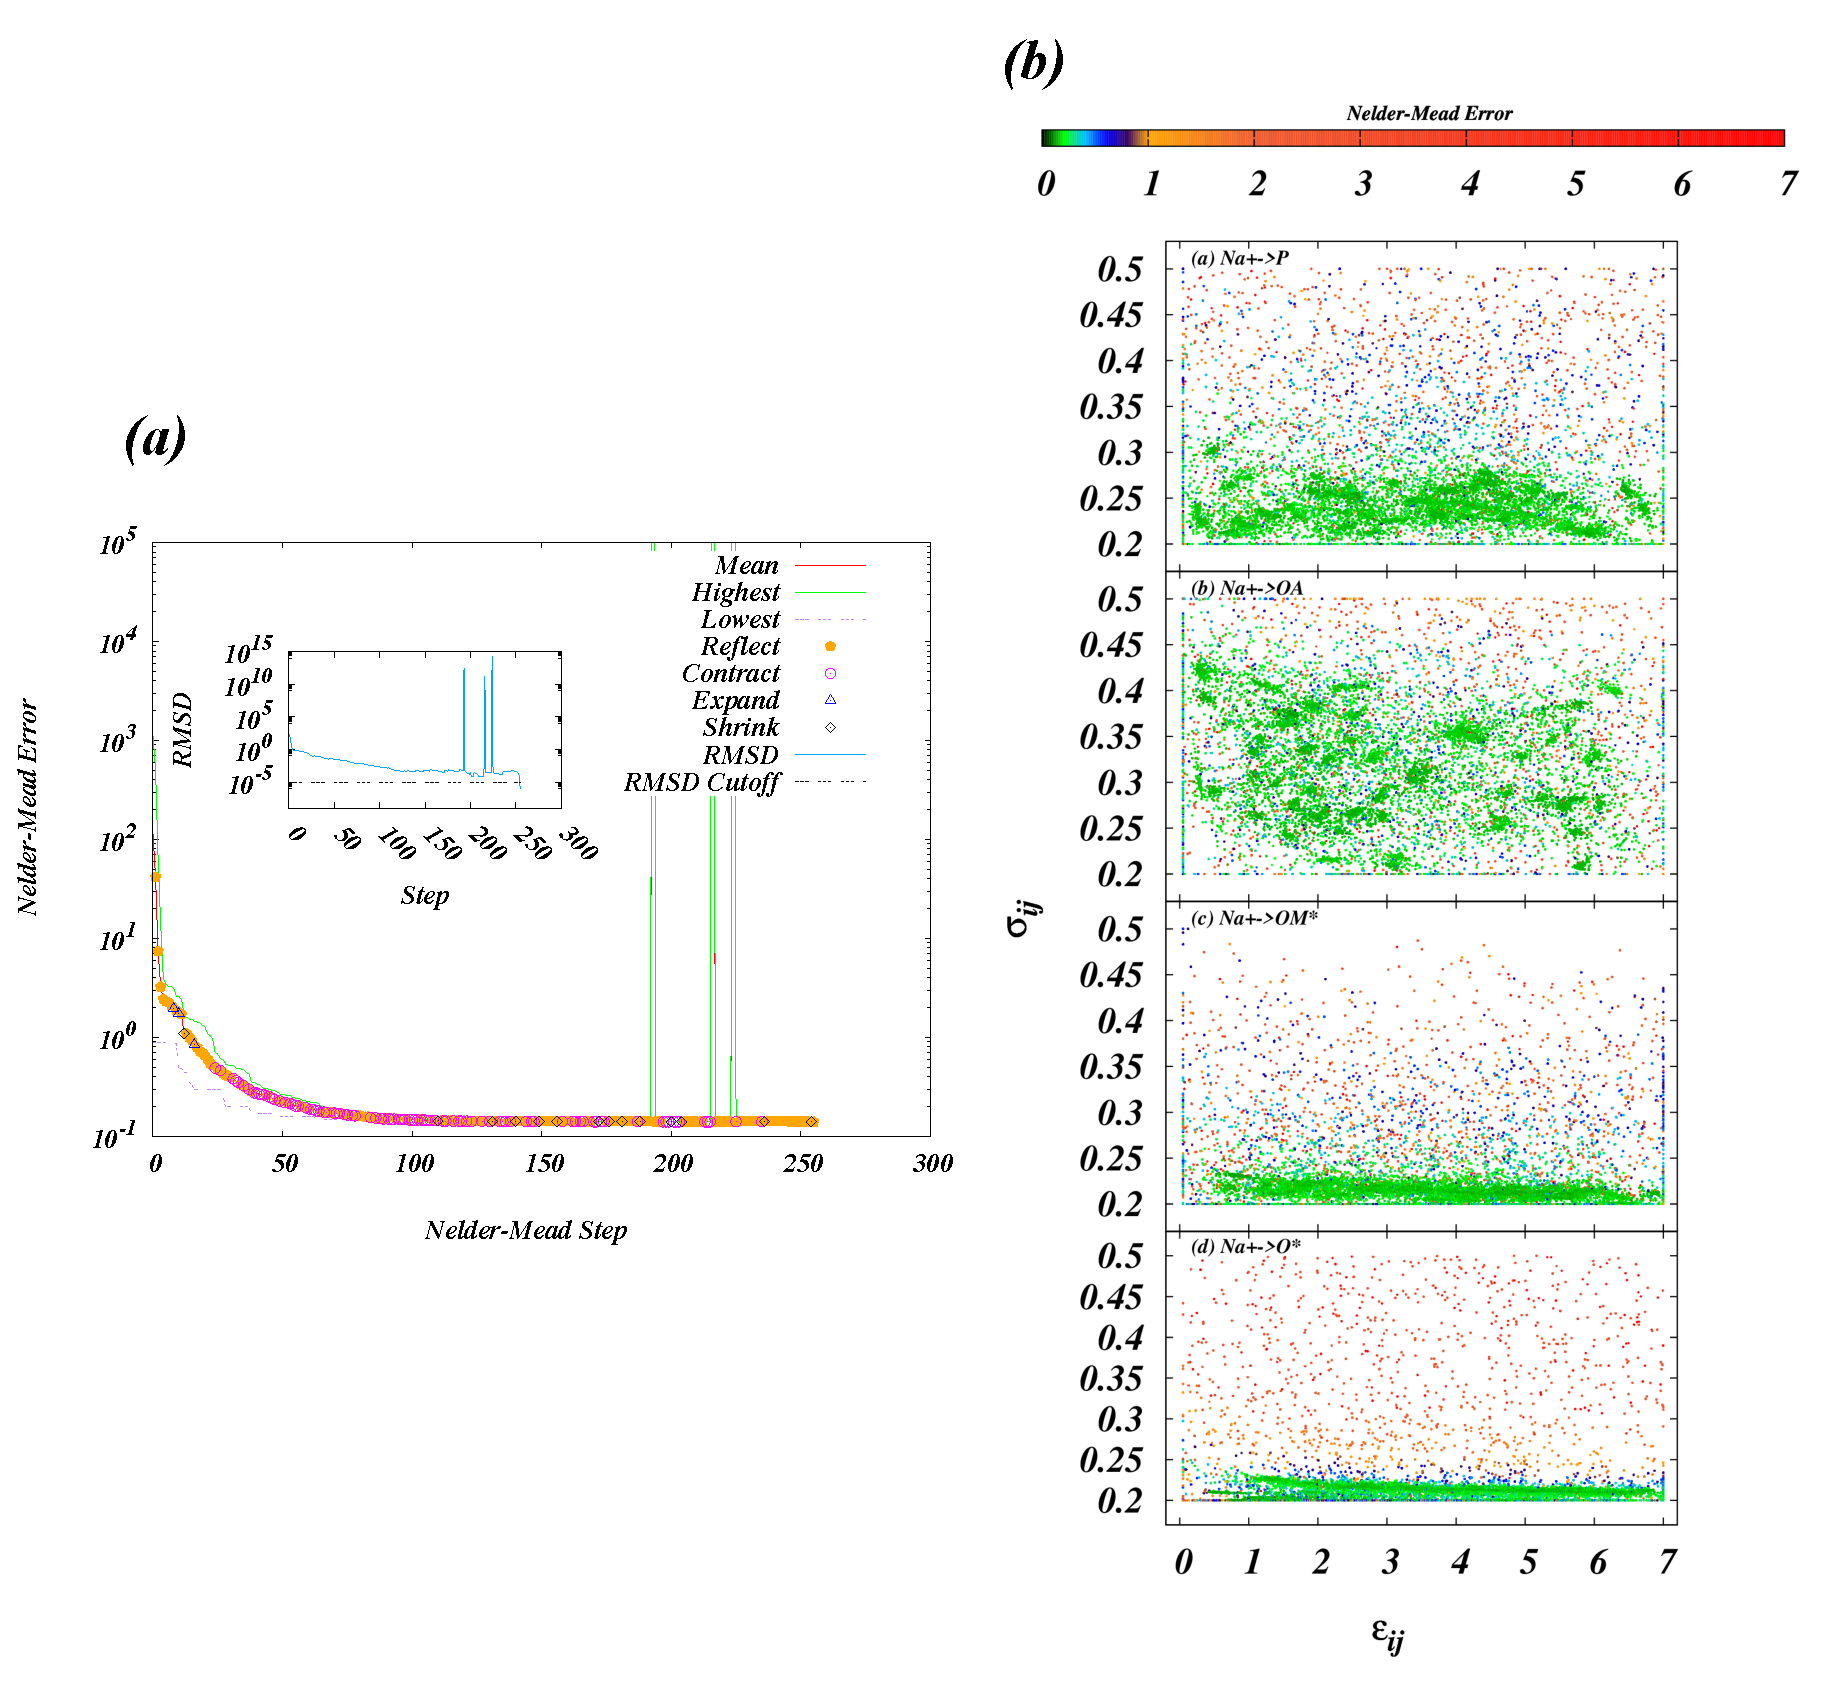
\includegraphics[width=\textwidth,trim=-3cm 0 0 -3cm]{figure_2.eps}
\end{figure}
\clearpage

\begin{figure}
    \caption{ }
    \label{fig:ioncoodcount}
    %\includegraphics[width=\textwidth,trim=-3cm 0 0 0]{ion_cood_count.eps}
    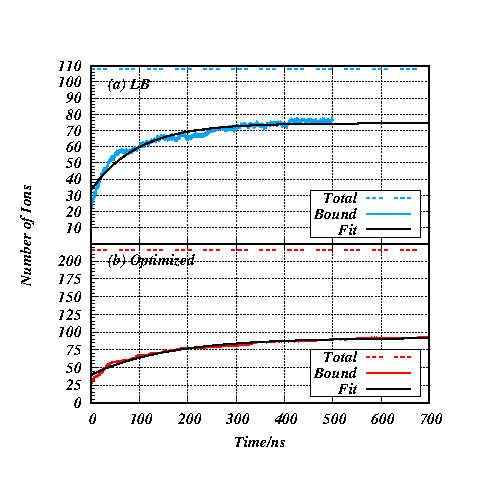
\includegraphics[width=\textwidth,trim=-3cm 0 0 0]{figure_3.eps}
    %RENAME n(t) to fit
\end{figure}
\clearpage
\begin{figure}[htb]
    \caption{ }
    \label{fig:eldens}
    %\includegraphics[width=\textwidth,trim=-3cm 0 0 0]{ele_dens.eps}
    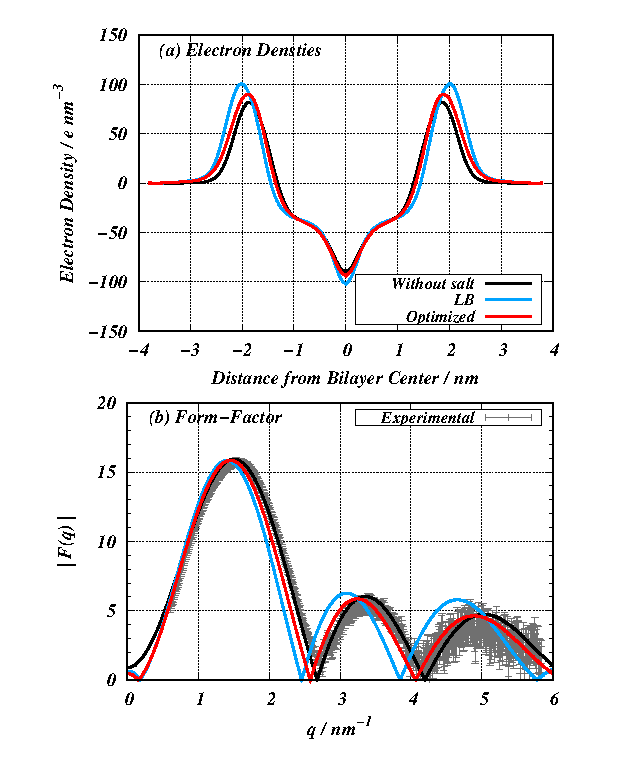
\includegraphics[width=\textwidth,trim=-3cm 0 0 0]{figure_4.eps}
\end{figure}
\clearpage
\begin{figure}[htb]
    \caption{ }
    \label{fig:cood}
    %\includegraphics[width=\textwidth,trim=-3cm 0 0 0]{cood.eps}
    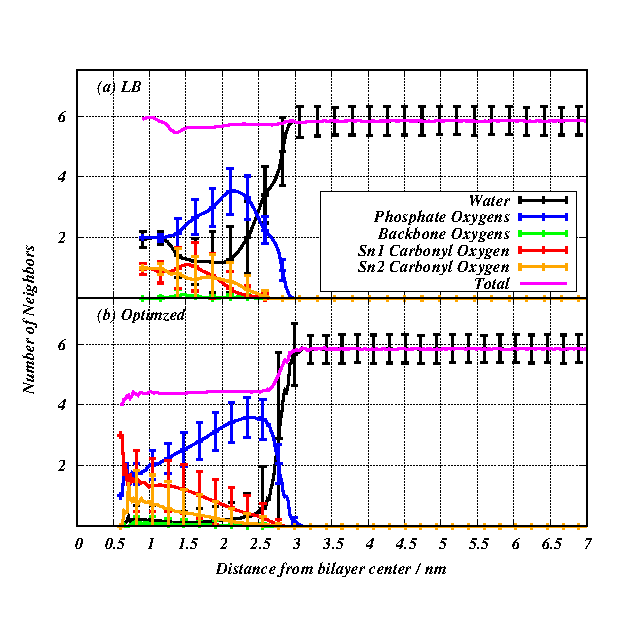
\includegraphics[width=\textwidth,trim=-3cm 0 0 0]{figure_5.eps}
\end{figure}
\clearpage
\clearpage
\begin{figure}[htb]
    \caption{ }
    \label{fig:waterdens}
    %\includegraphics[width=\textwidth,trim=-3cm 0 0 0]{dens_water.eps}
    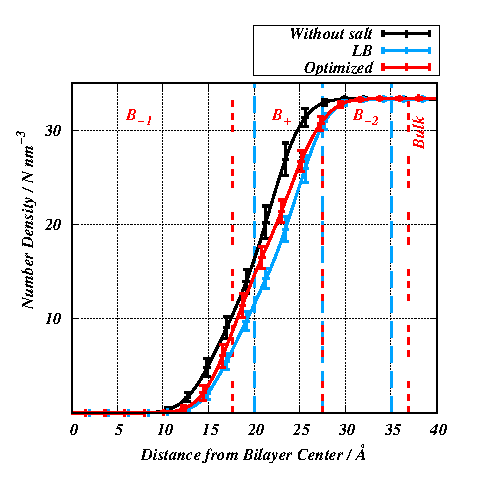
\includegraphics[width=\textwidth,trim=-3cm 0 0 0]{figure_6.eps}
\end{figure}
\clearpage
\begin{figure}[htb]
    \caption{ }
    \label{fig:waterorder}
    %\includegraphics[height=0.9\textheight,trim=-3cm -3cm 0 0]{h2order.eps}
    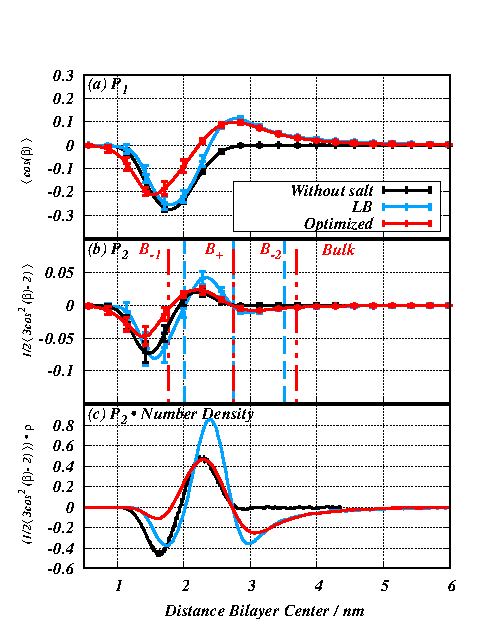
\includegraphics[height=0.9\textheight,trim=-3cm -3cm 0 0]{figure_7.eps}
    %SAME line thickness as others
\end{figure}
\clearpage
\clearpage


\end{document}
Workspace/refs.bib0000644000076500001200000021767414200525137014317 0ustar  msaundersadmin%% Created By Matthew Saunders for M.W.S. Thesis 2019 
%% Continued for IonOpt Paper M.W.S. 2020

@article{egberts:1988,
  title={Molecular dynamics simulation of a smectic liquid crystal with atomic detail},
  author={Egberts, E and Berendsen, HJC},
  journal={The Journal of chemical physics},
  volume={89},
  number={6},
  pages={3718--3732},
  year={1988},
  publisher={AIP}
}
@article{balleza:2014,
  title={Ether-versus ester-linked phospholipid bilayers containing either linear or branched apolar chains},
  author={Balleza, Daniel and Garcia-Arribas, Aritz B and Sot, Jes{\'u}s and Ruiz-Mirazo, Kepa and Go{\~n}i, F{\'e}lix M},
  journal={Biophysical journal},
  volume={107},
  number={6},
  pages={1364--1374},
  year={2014},
  publisher={Elsevier}
}
@article{klausg:1992,
  title={Membrane dipole potentials, hydration forces, and the ordering of water at membrane surfaces.},
  author={Gawrisch, K and Ruston, D and Zimmerberg, J and Parsegian, VA and Rand, RP and Fuller, N},
  journal={Biophysical journal},
  volume={61},
  number={5},
  pages={1213},
  year={1992},
  publisher={The Biophysical Society}
}
@article{guler:2009,
  title={Effects of ether vs. ester linkage on lipid bilayer structure and water permeability},
  author={Guler, S Deren and Ghosh, D Dipon and Pan, Jianjun and Mathai, John C and Zeidel, Mark L and Nagle, John F and Tristram-Nagle, Stephanie},
  journal={Chemistry and physics of lipids},
  volume={160},
  number={1},
  pages={33--44},
  year={2009},
  publisher={Elsevier}
}
@article{kruczek:2017,
author = {Kruczek, James and Chiu, See-Wing and Jakobsson, Eric and Pandit, Sagar A.},
title = {Effects of Lithium and Other Monovalent Ions on Palmitoyl Oleoyl Phosphatidylcholine Bilayer},
journal = {Langmuir},
volume = {33},
number = {4},
pages = {1105-1115},
year = {2017},
URL = {http://dx.doi.org/10.1021/acs.langmuir.6b04166},
}

@article{feller:1999,
  title={Constant surface tension simulations of lipid bilayers: the sensitivity of surface areas and compressibilities},
  author={Feller, Scott E and Pastor, Richard W},
  journal={The Journal of chemical physics},
  volume={111},
  number={3},
  pages={1281--1287},
  year={1999},
  publisher={AIP}
}


@incollection{Freitas:2016,
	Author = {Duarte Mota de Freitas and Brian D. Leverson and Jesse L. Goossens},
	Booktitle = {The alkali metal ions : their role for life},
	Chapter = {15},
	Date-Added = {2016-11-08 22:46:59 +0000},
	Date-Modified = {2016-11-08 23:00:11 +0000},
	Editor = {Astrid Sigel and Helmut Sigel and Roland K. O. Sigel},
	Pages = {557-584},
	Publisher = {Springer International Publishing},
	Title = {Lithium in Medicine: Mechanisms of Action},
	Volume = {16},
	Year = {2016}}

@article{fogarty:2015,
	Author = {Fogarty, Joseph C and Arjunwadkar, Mihir and Pandit, Sagar A and Pan, Jianjun},
	Journal = {Biochimica et Biophysica Acta (BBA)-Biomembranes},
	Number = {2},
	Pages = {662--672},
	Publisher = {Elsevier},
	Title = {Atomically detailed lipid bilayer models for the interpretation of small angle neutron and X-ray scattering data},
	Volume = {1848},
	Year = {2015}}

@article{gmx:1995,
	Author = {Berendsen, Herman JC and van der Spoel, David and van Drunen, Rudi},
	Date-Added = {2016-08-10 17:22:36 +0000},
	Date-Modified = {2016-08-10 17:23:01 +0000},
	Journal = {Computer Physics Communications},
	Number = {1},
	Pages = {43--56},
	Publisher = {Elsevier},
	Title = {GROMACS: a message-passing parallel molecular dynamics implementation},
	Volume = {91},
	Year = {1995}}

@article{gmx:2001,
	Author = {Lindahl, Erik and Hess, Berk and Van Der Spoel, David},
	Date-Added = {2016-08-10 17:21:03 +0000},
	Date-Modified = {2016-08-10 17:21:32 +0000},
	Journal = {Molecular modeling annual},
	Number = {8},
	Pages = {306--317},
	Publisher = {Springer},
	Title = {GROMACS 3.0: a package for molecular simulation and trajectory analysis},
	Volume = {7},
	Year = {2001}}

@article{gmx:2005,
	Author = {Van Der Spoel, David and Lindahl, Erik and Hess, Berk and Groenhof, Gerrit and Mark, Alan E and Berendsen, Herman JC},
	Date-Added = {2016-08-10 17:20:10 +0000},
	Date-Modified = {2016-08-10 17:20:36 +0000},
	Journal = {Journal of computational chemistry},
	Number = {16},
	Pages = {1701--1718},
	Publisher = {Wiley Online Library},
	Title = {GROMACS: fast, flexible, and free},
	Volume = {26},
	Year = {2005}}

@article{gmx:2008,
	Author = {Hess, Berk and Kutzner, Carsten and Van Der Spoel, David and Lindahl, Erik},
	Date-Added = {2016-08-10 17:18:15 +0000},
	Date-Modified = {2016-08-10 17:19:49 +0000},
	Journal = {Journal of chemical theory and computation},
	Number = {3},
	Pages = {435--447},
	Publisher = {ACS Publications},
	Title = {GROMACS 4: algorithms for highly efficient, load-balanced, and scalable molecular simulation},
	Volume = {4},
	Year = {2008}}

@article{Young:2008,
	Author = {Young, W},
	Date-Added = {2016-07-13 18:48:46 +0000},
	Date-Modified = {2016-07-13 18:49:12 +0000},
	Journal = {Cell transplantation},
	Number = {9},
	Pages = {951--975},
	Title = {Review of lithium effects on brain and blood.},
	Volume = {18},
	Year = {2008}}

@article{Sonne:2005,
	Author = {Sonne, Jacob and Hansen, Flemming Y. and Peters, G{\"u}nther H.},
	Date-Added = {2016-07-13 18:29:37 +0000},
	Date-Modified = {2016-07-13 18:41:44 +0000},
	Eid = 124903,
	Journal = {The Journal of Chemical Physics},
	Number = {12},
	Title = {Methodological problems in pressure profile calculations for lipid bilayers},
	Url = {http://scitation.aip.org/content/aip/journal/jcp/122/12/10.1063/1.1862624},
	Volume = {122},
	Year = {2005},
	Bdsk-Url-1 = {http://scitation.aip.org/content/aip/journal/jcp/122/12/10.1063/1.1862624},
	Bdsk-Url-2 = {http://dx.doi.org/10.1063/1.1862624}}

@article{Goetz:1998,
	Author = {Goetz, R and Lipowsky, R},
	Booktitle = {Journal of Chemical Physics},
	Date-Added = {2016-07-13 18:27:33 +0000},
	Date-Modified = {2016-07-13 19:01:23 +0000},
	Doi = {10.1063/1.476160},
	Isbn = {0021-9606},
	J2 = {J. Chem. Phys.},
	Journal = {Journal of Chemical Physics},
	Keywords = {MOLECULAR-DYNAMICS SIMULATION; LIQUID-CRYSTAL; MONOLAYER},
	La = {English},
	Number = {17},
	Pages = {7397--7409},
	Title = {Computer simulations of bilayer membranes : Self-assembly and interfacial tension},
	Ty = {JOUR},
	Url = {http://www.cheric.org/research/tech/periodicals/view.php?seq=121428},
	Volume = {108},
	Year = {1998},
	Bdsk-File-1 = {YnBsaXN0MDDUAQIDBAUGJCVYJHZlcnNpb25YJG9iamVjdHNZJGFyY2hpdmVyVCR0b3ASAAGGoKgHCBMUFRYaIVUkbnVsbNMJCgsMDxJXTlMua2V5c1pOUy5vYmplY3RzViRjbGFzc6INDoACgAOiEBGABIAFgAdccmVsYXRpdmVQYXRoWWFsaWFzRGF0YV8QdS4uLy4uLy4uLy4uLy4uL0hvbWUvamtydWN6ZWsvRHJvcGJveC9KYW1lc19QSEQvU3VyZmFjZSBUZW5zaW9uL0dvZXR6X1JfTGlwb3dza3lfUl9Db21wdXRlcl9zaW11bGF0aW9uc19vZl9iaWxheWVyLnBkZtIXCxgZV05TLmRhdGFPEQIyAAAAAAIyAAIAAARIb21lAAAAAAAAAAAAAAAAAAAAAAAAAAAAAAAAAAAATkoAAf////8fR29ldHpfUl9MaXBvd3NreV9SI0ZGRkZGRkZGLnBkZgAAAAAAAAAAAAAAAAAAAAAAAAAAAAAAAAAAAAAAAAAA/////wAAAAAAAAAAAAAAAP////8AABKBY3UAAAAAAAAAAAAAAAAAD1N1cmZhY2UgVGVuc2lvbgAAAgBsLzptbnQ6SG9tZTpqa3J1Y3plazpEcm9wYm94OkphbWVzX1BIRDpTdXJmYWNlIFRlbnNpb246R29ldHpfUl9MaXBvd3NreV9SX0NvbXB1dGVyX3NpbXVsYXRpb25zX29mX2JpbGF5ZXIucGRmAA4AbgA2AEcAbwBlAHQAegBfAFIAXwBMAGkAcABvAHcAcwBrAHkAXwBSAF8AQwBvAG0AcAB1AHQAZQByAF8AcwBpAG0AdQBsAGEAdABpAG8AbgBzAF8AbwBmAF8AYgBpAGwAYQB5AGUAcgAuAHAAZABmAA8ACgAEAEgAbwBtAGUAEgBiL2prcnVjemVrL0Ryb3Bib3gvSmFtZXNfUEhEL1N1cmZhY2UgVGVuc2lvbi9Hb2V0el9SX0xpcG93c2t5X1JfQ29tcHV0ZXJfc2ltdWxhdGlvbnNfb2ZfYmlsYXllci5wZGYAEwAJL21udC9Ib21lAAAJABYAFmNyYm0AAHBvc3gvbW50L0hvbWUAABUAAgAS//8AAIAG0hscHR5aJGNsYXNzbmFtZVgkY2xhc3Nlc11OU011dGFibGVEYXRhox0fIFZOU0RhdGFYTlNPYmplY3TSGxwiI1xOU0RpY3Rpb25hcnmiIiBfEA9OU0tleWVkQXJjaGl2ZXLRJidUcm9vdIABAAgAEQAaACMALQAyADcAQABGAE0AVQBgAGcAagBsAG4AcQBzAHUAdwCEAI4BBgELARMDSQNLA1ADWwNkA3IDdgN9A4YDiwOYA5sDrQOwA7UAAAAAAAACAQAAAAAAAAAoAAAAAAAAAAAAAAAAAAADtw==}}

@article{Jahnig:1996,
	Author = {Jahnig, F},
	Date-Added = {2016-07-13 18:21:59 +0000},
	Date-Modified = {2016-07-13 18:42:38 +0000},
	Issn = {{0006-3495}},
	Journal = {{BIOPHYSICAL JOURNAL}},
	Month = {{SEP}},
	Number = {{3}},
	Pages = {{1348-1349}},
	Title = {{What is the surface tension of a lipid bilayer membrane?}},
	Unique-Id = {{ISI:A1996VF09700021}},
	Volume = {{71}},
	Year = {{1996}}}

@article{petrache:1997,
	Abstract = {An efficient method for extracting volumetric data from simulations is developed. The method is illustrated using a recent atomic-level molecular dynamics simulation of L alpha phase 1,2-dipalmitoyl-sn-glycero-3-phosphocholine bilayer. Results from this simulation are obtained for the volumes of water (VW), lipid (V1), chain methylenes (V2), chain terminal methyls (V3), and lipid headgroups (VH), including separate volumes for carboxyl (Vcoo), glyceryl (Vgl), phosphoryl (VPO4), and choline (Vchol) groups. The method assumes only that each group has the same average volume regardless of its location in the bilayer, and this assumption is then tested with the current simulation. The volumes obtained agree well with the values VW and VL that have been obtained directly from experiment, as well as with the volumes VH, V2, and V3 that require certain assumptions in addition to the experimental data. This method should help to support and refine some assumptions that are necessary when interpreting experimental data. IMAGES:},
	An = {PMC1184418},
	Author = {Petrache, H I and Feller, S E and Nagle, J F},
	Date = {1997/05/},
	Date-Added = {2016-07-13 18:14:45 +0000},
	Date-Modified = {2016-07-13 18:35:22 +0000},
	Db = {PMC},
	Isbn = {0006-3495; 1542-0086},
	J1 = {Biophys J},
	Journal = {Biophysical Journal},
	Month = {05},
	Number = {5},
	Pages = {2237--2242},
	Title = {Determination of component volumes of lipid bilayers from simulations.},
	Ty = {JOUR},
	U1 = {9129826{$[$}pmid{$]$}; 9129826{$[$}pmid{$]$}},
	Url = {http://www.ncbi.nlm.nih.gov/pmc/articles/PMC1184418/},
	Volume = {72},
	Year = {1997},
	Bdsk-Url-1 = {http://www.ncbi.nlm.nih.gov/pmc/articles/PMC1184418/}}

@article{Berkowitz:2006,
	Author = {Berkowitz, Max L and Bostick, David L and Pandit, Sagar},
	Date-Added = {2016-07-13 18:07:17 +0000},
	Date-Modified = {2016-07-13 18:33:52 +0000},
	Journal = {Chemical reviews},
	Number = {4},
	Pages = {1527--1539},
	Publisher = {ACS Publications},
	Title = {Aqueous solutions next to phospholipid membrane surfaces: insights from simulations},
	Volume = {106},
	Year = {2006},
	Bdsk-File-1 = {YnBsaXN0MDDUAQIDBAUGJCVYJHZlcnNpb25YJG9iamVjdHNZJGFyY2hpdmVyVCR0b3ASAAGGoKgHCBMUFRYaIVUkbnVsbNMJCgsMDxJXTlMua2V5c1pOUy5vYmplY3RzViRjbGFzc6INDoACgAOiEBGABIAFgAdccmVsYXRpdmVQYXRoWWFsaWFzRGF0YV8QTi4uLy4uLy4uLy4uLy4uL0hvbWUvamtydWN6ZWsvRHJvcGJveC9KYW1lc19QSEQvSW9ucy9zYWdhci1jaGVtLXJldmlldy0yMDA2LnBkZtIXCxgZV05TLmRhdGFPEQGiAAAAAAGiAAIAAARIb21lAAAAAAAAAAAAAAAAAAAAAAAAAAAAAAAAAAAATkoAAf////8ac2FnYXItY2hlbS1yZXZpZXctMjAwNi5wZGYAAAAAAAAAAAAAAAAAAAAAAAAAAAAAAAAAAAAAAAAAAAAAAAAA/////wAAAAAAAAAAAAAAAP////8AABKBY3UAAAAAAAAAAAAAAAAABElvbnMAAgBFLzptbnQ6SG9tZTpqa3J1Y3plazpEcm9wYm94OkphbWVzX1BIRDpJb25zOnNhZ2FyLWNoZW0tcmV2aWV3LTIwMDYucGRmAAAOADYAGgBzAGEAZwBhAHIALQBjAGgAZQBtAC0AcgBlAHYAaQBlAHcALQAyADAAMAA2AC4AcABkAGYADwAKAAQASABvAG0AZQASADsvamtydWN6ZWsvRHJvcGJveC9KYW1lc19QSEQvSW9ucy9zYWdhci1jaGVtLXJldmlldy0yMDA2LnBkZgAAEwAJL21udC9Ib21lAAAJABYAFmNyYm0AAHBvc3gvbW50L0hvbWUAABUAAgAS//8AAIAG0hscHR5aJGNsYXNzbmFtZVgkY2xhc3Nlc11OU011dGFibGVEYXRhox0fIFZOU0RhdGFYTlNPYmplY3TSGxwiI1xOU0RpY3Rpb25hcnmiIiBfEA9OU0tleWVkQXJjaGl2ZXLRJidUcm9vdIABAAgAEQAaACMALQAyADcAQABGAE0AVQBgAGcAagBsAG4AcQBzAHUAdwCEAI4A3wDkAOwCkgKUApkCpAKtArsCvwLGAs8C1ALhAuQC9gL5Av4AAAAAAAACAQAAAAAAAAAoAAAAAAAAAAAAAAAAAAADAA==}}

@article{joung:2008,
	Author = {Joung, In Suk and Cheatham III, Thomas E},
	Date-Added = {2016-07-13 18:06:44 +0000},
	Date-Modified = {2016-07-13 18:35:05 +0000},
	Journal = {The journal of physical chemistry B},
	Number = {30},
	Pages = {9020--9041},
	Publisher = {ACS Publications},
	Title = {Determination of alkali and halide monovalent ion parameters for use in explicitly solvated biomolecular simulations},
	Volume = {112},
	Year = {2008},
	Bdsk-File-1 = {YnBsaXN0MDDUAQIDBAUGJCVYJHZlcnNpb25YJG9iamVjdHNZJGFyY2hpdmVyVCR0b3ASAAGGoKgHCBMUFRYaIVUkbnVsbNMJCgsMDxJXTlMua2V5c1pOUy5vYmplY3RzViRjbGFzc6INDoACgAOiEBGABIAFgAdccmVsYXRpdmVQYXRoWWFsaWFzRGF0YV8QPi4uLy4uLy4uLy4uLy4uL0hvbWUvamtydWN6ZWsvRHJvcGJveC9KYW1lc19QSEQvSW9ucy9Kb3VuZ3MucGRm0hcLGBlXTlMuZGF0YU8RAWIAAAAAAWIAAgAABEhvbWUAAAAAAAAAAAAAAAAAAAAAAAAAAAAAAAAAAABOSgAB/////wpKb3VuZ3MucGRmAAAAAAAAAAAAAAAAAAAAAAAAAAAAAAAAAAAAAAAAAAAAAAAAAAAAAAAAAAAAAAAAAAAAAAD/////AAAAAAAAAAAAAAAA/////wAAEoFjdQAAAAAAAAAAAAAAAAAESW9ucwACADUvOm1udDpIb21lOmprcnVjemVrOkRyb3Bib3g6SmFtZXNfUEhEOklvbnM6Sm91bmdzLnBkZgAADgAWAAoASgBvAHUAbgBnAHMALgBwAGQAZgAPAAoABABIAG8AbQBlABIAKy9qa3J1Y3play9Ecm9wYm94L0phbWVzX1BIRC9Jb25zL0pvdW5ncy5wZGYAABMACS9tbnQvSG9tZQAACQAWABZjcmJtAABwb3N4L21udC9Ib21lAAAVAAIAEv//AACABtIbHB0eWiRjbGFzc25hbWVYJGNsYXNzZXNdTlNNdXRhYmxlRGF0YaMdHyBWTlNEYXRhWE5TT2JqZWN00hscIiNcTlNEaWN0aW9uYXJ5oiIgXxAPTlNLZXllZEFyY2hpdmVy0SYnVHJvb3SAAQAIABEAGgAjAC0AMgA3AEAARgBNAFUAYABnAGoAbABuAHEAcwB1AHcAhACOAM8A1ADcAkICRAJJAlQCXQJrAm8CdgJ/AoQCkQKUAqYCqQKuAAAAAAAAAgEAAAAAAAAAKAAAAAAAAAAAAAAAAAAAArA=}}

@article{Binder:2002,
	Author = {Binder, Hans and Zsch{\"o}rnig, Olaf},
	Date-Added = {2016-07-13 18:06:13 +0000},
	Date-Modified = {2016-07-13 18:42:09 +0000},
	Journal = {Chemistry and physics of lipids},
	Number = {1},
	Pages = {39--61},
	Publisher = {Elsevier},
	Title = {The effect of metal cations on the phase behavior and hydration characteristics of phospholipid membranes},
	Volume = {115},
	Year = {2002}}

@article{Akutsu:1981,
	Author = {Akutsu, Hideo and Seelig, Joachim},
	Date-Added = {2016-07-13 18:05:17 +0000},
	Date-Modified = {2016-07-13 18:41:14 +0000},
	Journal = {Biochemistry},
	Number = {26},
	Pages = {7366--7373},
	Publisher = {ACS Publications},
	Title = {Interaction of metal ions with phosphatidylcholine bilayer membranes},
	Volume = {20},
	Year = {1981}}

@article{Cordomi:2008,
	Author = {Cordomi, Arnau and Edholm, Olle and Perez, Juan J},
	Date-Added = {2016-07-13 18:04:28 +0000},
	Date-Modified = {2016-07-13 18:39:47 +0000},
	Journal = {The Journal of Physical Chemistry B},
	Number = {5},
	Pages = {1397--1408},
	Publisher = {ACS Publications},
	Title = {Effect of ions on a dipalmitoyl phosphatidylcholine bilayer. A molecular dynamics simulation study},
	Volume = {112},
	Year = {2008},
	Bdsk-File-1 = {YnBsaXN0MDDUAQIDBAUGJCVYJHZlcnNpb25YJG9iamVjdHNZJGFyY2hpdmVyVCR0b3ASAAGGoKgHCBMUFRYaIVUkbnVsbNMJCgsMDxJXTlMua2V5c1pOUy5vYmplY3RzViRjbGFzc6INDoACgAOiEBGABIAFgAdccmVsYXRpdmVQYXRoWWFsaWFzRGF0YV8QSS4uLy4uLy4uLy4uLy4uL0hvbWUvamtydWN6ZWsvRHJvcGJveC9KYW1lc19QSEQvSW9ucy9Bcm5hdV9Gb3JjZV9GaWVsZC5wZGbSFwsYGVdOUy5kYXRhTxEBjAAAAAABjAACAAAESG9tZQAAAAAAAAAAAAAAAAAAAAAAAAAAAAAAAAAAAE5KAAH/////FUFybmF1X0ZvcmNlX0ZpZWxkLnBkZgAAAAAAAAAAAAAAAAAAAAAAAAAAAAAAAAAAAAAAAAAAAAAAAAAAAAAAAP////8AAAAAAAAAAAAAAAD/////AAASgWN1AAAAAAAAAAAAAAAAAARJb25zAAIAQC86bW50OkhvbWU6amtydWN6ZWs6RHJvcGJveDpKYW1lc19QSEQ6SW9uczpBcm5hdV9Gb3JjZV9GaWVsZC5wZGYADgAsABUAQQByAG4AYQB1AF8ARgBvAHIAYwBlAF8ARgBpAGUAbABkAC4AcABkAGYADwAKAAQASABvAG0AZQASADYvamtydWN6ZWsvRHJvcGJveC9KYW1lc19QSEQvSW9ucy9Bcm5hdV9Gb3JjZV9GaWVsZC5wZGYAEwAJL21udC9Ib21lAAAJABYAFmNyYm0AAHBvc3gvbW50L0hvbWUAABUAAgAS//8AAIAG0hscHR5aJGNsYXNzbmFtZVgkY2xhc3Nlc11OU011dGFibGVEYXRhox0fIFZOU0RhdGFYTlNPYmplY3TSGxwiI1xOU0RpY3Rpb25hcnmiIiBfEA9OU0tleWVkQXJjaGl2ZXLRJidUcm9vdIABAAgAEQAaACMALQAyADcAQABGAE0AVQBgAGcAagBsAG4AcQBzAHUAdwCEAI4A2gDfAOcCdwJ5An4CiQKSAqACpAKrArQCuQLGAskC2wLeAuMAAAAAAAACAQAAAAAAAAAoAAAAAAAAAAAAAAAAAAAC5Q==}}

@article{Cordomi:2009,
	Author = {Cordomi, Arnau and Edholm, Olle and Perez, Juan J},
	Date-Added = {2016-07-13 18:04:03 +0000},
	Date-Modified = {2016-07-13 18:39:27 +0000},
	Journal = {Journal of chemical theory and computation},
	Number = {8},
	Pages = {2125--2134},
	Publisher = {ACS Publications},
	Title = {Effect of force field parameters on sodium and potassium ion binding to dipalmitoyl phosphatidylcholine bilayers},
	Volume = {5},
	Year = {2009},
	Bdsk-File-1 = {YnBsaXN0MDDUAQIDBAUGJCVYJHZlcnNpb25YJG9iamVjdHNZJGFyY2hpdmVyVCR0b3ASAAGGoKgHCBMUFRYaIVUkbnVsbNMJCgsMDxJXTlMua2V5c1pOUy5vYmplY3RzViRjbGFzc6INDoACgAOiEBGABIAFgAdccmVsYXRpdmVQYXRoWWFsaWFzRGF0YV8QSS4uLy4uLy4uLy4uLy4uL0hvbWUvamtydWN6ZWsvRHJvcGJveC9KYW1lc19QSEQvSW9ucy9Bcm5hdV9Gb3JjZV9GaWVsZC5wZGbSFwsYGVdOUy5kYXRhTxEBjAAAAAABjAACAAAESG9tZQAAAAAAAAAAAAAAAAAAAAAAAAAAAAAAAAAAAE5KAAH/////FUFybmF1X0ZvcmNlX0ZpZWxkLnBkZgAAAAAAAAAAAAAAAAAAAAAAAAAAAAAAAAAAAAAAAAAAAAAAAAAAAAAAAP////8AAAAAAAAAAAAAAAD/////AAASgWN1AAAAAAAAAAAAAAAAAARJb25zAAIAQC86bW50OkhvbWU6amtydWN6ZWs6RHJvcGJveDpKYW1lc19QSEQ6SW9uczpBcm5hdV9Gb3JjZV9GaWVsZC5wZGYADgAsABUAQQByAG4AYQB1AF8ARgBvAHIAYwBlAF8ARgBpAGUAbABkAC4AcABkAGYADwAKAAQASABvAG0AZQASADYvamtydWN6ZWsvRHJvcGJveC9KYW1lc19QSEQvSW9ucy9Bcm5hdV9Gb3JjZV9GaWVsZC5wZGYAEwAJL21udC9Ib21lAAAJABYAFmNyYm0AAHBvc3gvbW50L0hvbWUAABUAAgAS//8AAIAG0hscHR5aJGNsYXNzbmFtZVgkY2xhc3Nlc11OU011dGFibGVEYXRhox0fIFZOU0RhdGFYTlNPYmplY3TSGxwiI1xOU0RpY3Rpb25hcnmiIiBfEA9OU0tleWVkQXJjaGl2ZXLRJidUcm9vdIABAAgAEQAaACMALQAyADcAQABGAE0AVQBgAGcAagBsAG4AcQBzAHUAdwCEAI4A2gDfAOcCdwJ5An4CiQKSAqACpAKrArQCuQLGAskC2wLeAuMAAAAAAAACAQAAAAAAAAAoAAAAAAAAAAAAAAAAAAAC5Q==}}

@article{Bockmann:2003,
	Author = {B{\"o}ckmann, Rainer A and Hac, Agnieszka and Heimburg, Thomas and Grubm{\"u}ller, Helmut},
	Date-Added = {2016-07-13 18:03:27 +0000},
	Date-Modified = {2016-07-13 18:40:34 +0000},
	Journal = {Biophysical Journal},
	Number = {3},
	Pages = {1647--1655},
	Publisher = {Elsevier},
	Title = {Effect of sodium chloride on a lipid bilayer},
	Volume = {85},
	Year = {2003}}


@article{Lindahl:2000,
	Author = {Lindahl, Erik and Edholm, Olle},
	Date-Added = {2016-07-13 17:15:27 +0000},
	Date-Modified = {2016-07-13 17:36:08 +0000},
	Journal = {The Journal of Chemical Physics},
	Number = {9},
	Pages = {3882--3893},
	Publisher = {AIP Publishing},
	Title = {Spatial and energetic-entropic decomposition of surface tension in lipid bilayers from molecular dynamics simulations},
	Volume = {113},
	Year = {2000},
	Bdsk-File-1 = {YnBsaXN0MDDUAQIDBAUGJCVYJHZlcnNpb25YJG9iamVjdHNZJGFyY2hpdmVyVCR0b3ASAAGGoKgHCBMUFRYaIVUkbnVsbNMJCgsMDxJXTlMua2V5c1pOUy5vYmplY3RzViRjbGFzc6INDoACgAOiEBGABIAFgAdccmVsYXRpdmVQYXRoWWFsaWFzRGF0YV8QWS4uLy4uLy4uLy4uLy4uL0hvbWUvamtydWN6ZWsvRHJvcGJveC9KYW1lc19QSEQvU3VyZmFjZSBUZW5zaW9uL0xpbmRhbC1FZGhvbG0tcHJlc3N1cmUucGRm0hcLGBlXTlMuZGF0YU8RAcIAAAAAAcIAAgAABEhvbWUAAAAAAAAAAAAAAAAAAAAAAAAAAAAAAAAAAABOSgAB/////xpMaW5kYWwtRWRob2xtLXByZXNzdXJlLnBkZgAAAAAAAAAAAAAAAAAAAAAAAAAAAAAAAAAAAAAAAAAAAAAAAAD/////AAAAAAAAAAAAAAAA/////wAAEoFjdQAAAAAAAAAAAAAAAAAPU3VyZmFjZSBUZW5zaW9uAAACAFAvOm1udDpIb21lOmprcnVjemVrOkRyb3Bib3g6SmFtZXNfUEhEOlN1cmZhY2UgVGVuc2lvbjpMaW5kYWwtRWRob2xtLXByZXNzdXJlLnBkZgAOADYAGgBMAGkAbgBkAGEAbAAtAEUAZABoAG8AbABtAC0AcAByAGUAcwBzAHUAcgBlAC4AcABkAGYADwAKAAQASABvAG0AZQASAEYvamtydWN6ZWsvRHJvcGJveC9KYW1lc19QSEQvU3VyZmFjZSBUZW5zaW9uL0xpbmRhbC1FZGhvbG0tcHJlc3N1cmUucGRmABMACS9tbnQvSG9tZQAACQAWABZjcmJtAABwb3N4L21udC9Ib21lAAAVAAIAEv//AACABtIbHB0eWiRjbGFzc25hbWVYJGNsYXNzZXNdTlNNdXRhYmxlRGF0YaMdHyBWTlNEYXRhWE5TT2JqZWN00hscIiNcTlNEaWN0aW9uYXJ5oiIgXxAPTlNLZXllZEFyY2hpdmVy0SYnVHJvb3SAAQAIABEAGgAjAC0AMgA3AEAARgBNAFUAYABnAGoAbABuAHEAcwB1AHcAhACOAOoA7wD3Ar0CvwLEAs8C2ALmAuoC8QL6Av8DDAMPAyEDJAMpAAAAAAAAAgEAAAAAAAAAKAAAAAAAAAAAAAAAAAAAAys=}}

@article{Vanegas:2014,
	Author = {Vanegas, Juan M and Torres-S{\'a}nchez, Alejandro and Arroyo, Marino},
	Date-Added = {2016-07-13 17:14:49 +0000},
	Date-Modified = {2016-07-13 17:36:22 +0000},
	Journal = {Journal of chemical theory and computation},
	Number = {2},
	Pages = {691--702},
	Publisher = {ACS Publications},
	Title = {Importance of force decomposition for local stress calculations in biomembrane molecular simulations},
	Volume = {10},
	Year = {2014},
	Bdsk-File-1 = {YnBsaXN0MDDUAQIDBAUGJCVYJHZlcnNpb25YJG9iamVjdHNZJGFyY2hpdmVyVCR0b3ASAAGGoKgHCBMUFRYaIVUkbnVsbNMJCgsMDxJXTlMua2V5c1pOUy5vYmplY3RzViRjbGFzc6INDoACgAOiEBGABIAFgAdccmVsYXRpdmVQYXRoWWFsaWFzRGF0YV8QYS4uLy4uLy4uLy4uLy4uL0hvbWUvamtydWN6ZWsvRHJvcGJveC9KYW1lc19QSEQvU3VyZmFjZSBUZW5zaW9uL2xvY2FsLXN0cmVzcy1ncm9hbWNzLWNvZGUtZ3V5cy5wZGbSFwsYGVdOUy5kYXRhTxEB4gAAAAAB4gACAAAESG9tZQAAAAAAAAAAAAAAAAAAAAAAAAAAAAAAAAAAAE5KAAH/////H2xvY2FsLXN0cmVzcy1ncm9hbSNGRkZGRkZGRi5wZGYAAAAAAAAAAAAAAAAAAAAAAAAAAAAAAAAAAAAAAAAAAP////8AAAAAAAAAAAAAAAD/////AAASgWN1AAAAAAAAAAAAAAAAAA9TdXJmYWNlIFRlbnNpb24AAAIAWC86bW50OkhvbWU6amtydWN6ZWs6RHJvcGJveDpKYW1lc19QSEQ6U3VyZmFjZSBUZW5zaW9uOmxvY2FsLXN0cmVzcy1ncm9hbWNzLWNvZGUtZ3V5cy5wZGYADgBGACIAbABvAGMAYQBsAC0AcwB0AHIAZQBzAHMALQBnAHIAbwBhAG0AYwBzAC0AYwBvAGQAZQAtAGcAdQB5AHMALgBwAGQAZgAPAAoABABIAG8AbQBlABIATi9qa3J1Y3play9Ecm9wYm94L0phbWVzX1BIRC9TdXJmYWNlIFRlbnNpb24vbG9jYWwtc3RyZXNzLWdyb2FtY3MtY29kZS1ndXlzLnBkZgATAAkvbW50L0hvbWUAAAkAFgAWY3JibQAAcG9zeC9tbnQvSG9tZQAAFQACABL//wAAgAbSGxwdHlokY2xhc3NuYW1lWCRjbGFzc2VzXU5TTXV0YWJsZURhdGGjHR8gVk5TRGF0YVhOU09iamVjdNIbHCIjXE5TRGljdGlvbmFyeaIiIF8QD05TS2V5ZWRBcmNoaXZlctEmJ1Ryb290gAEACAARABoAIwAtADIANwBAAEYATQBVAGAAZwBqAGwAbgBxAHMAdQB3AIQAjgDyAPcA/wLlAucC7AL3AwADDgMSAxkDIgMnAzQDNwNJA0wDUQAAAAAAAAIBAAAAAAAAACgAAAAAAAAAAAAAAAAAAANT}}

@article{lincs,
	Author = {Hess, Berk and Bekker, Henk and Berendsen, Herman J. C. and Fraaije, Johannes G. E. M.},
	Issn = {1096-987X},
	Journal = {Journal of Computational Chemistry},
	Keywords = {constraints, molecular dynamics, Langevin dynamics, SHAKE},
	Number = {12},
	Pages = {1463--1472},
	Publisher = {John Wiley & Sons, Inc.},
	Title = {LINCS: A linear constraint solver for molecular simulations},
	Url = {http://dx.doi.org/10.1002/(SICI)1096-987X(199709)18:12<1463::AID-JCC4>3.0.CO;2-H},
	Volume = {18},
	Year = {1997}
}

@article{pme:1995,
	Author = {Essmann, Ulrich and Perera, Lalith and Berkowitz, Max L and Darden, Tom and Lee, Hsing and Pedersen, Lee G},
	Journal = {The Journal of chemical physics},
	Number = {19},
	Pages = {8577--8593},
	Publisher = {AIP Publishing},
	Title = {A smooth particle mesh Ewald method},
	Volume = {103},
	Year = {1995}}

@article{nose:1983,
	Author = {Nos{\'e}, Shuichi and Klein, ML},
	Journal = {Molecular Physics},
	Number = {5},
	Pages = {1055--1076},
	Publisher = {Taylor \& Francis},
	Title = {Constant pressure molecular dynamics for molecular systems},
	Volume = {50},
	Year = {1983}}

@article{parrinello:1981,
	Author = {Parrinello, Michele and Rahman, Aneesur},
	Journal = {Journal of Applied physics},
	Number = {12},
	Pages = {7182--7190},
	Publisher = {AIP Publishing},
	Title = {Polymorphic transitions in single crystals: A new molecular dynamics method},
	Volume = {52},
	Year = {1981}}

@article{klein:1996,
	Author = {Klein, Peter S and Melton, Douglas A},
	Journal = {Proceedings of the National Academy of Sciences},
	Number = {16},
	Pages = {8455--8459},
	Publisher = {National Acad Sciences},
	Title = {A molecular mechanism for the effect of lithium on development},
	Volume = {93},
	Year = {1996}}

@article{stambolic:1996,
	Author = {Stambolic, Vuk and Ruel, Laurent and Woodgett, James R},
	Journal = {Current Biology},
	Number = {12},
	Pages = {1664--1669},
	Publisher = {Elsevier},
	Title = {Lithium inhibits glycogen synthase kinase-3 activity and mimics wingless signalling in intact cells},
	Volume = {6},
	Year = {1996}}

@article{cade:1949,
	Author = {Cade, John FJ},
	Journal = {Medical Journal of Australia},
	Publisher = {Australasian Medical Publishing Company, Limited},
	Title = {Lithium salts in the treatment of psychotic excitement.},
	Year = {1949}}

@article{sarkar:2005,
	Author = {Sarkar, Sovan and Floto, R Andres and Berger, Zdenek and Imarisio, Sara and Cordenier, Axelle and Pasco, Matthieu and Cook, Lynnette J and Rubinsztein, David C},
	Journal = {The Journal of cell biology},
	Number = {7},
	Pages = {1101--1111},
	Publisher = {Rockefeller Univ Press},
	Title = {Lithium induces autophagy by inhibiting inositol monophosphatase},
	Volume = {170},
	Year = {2005}}

@article{atack:1993,
	Author = {Atack, John R and Cook, Susan M and Watt, Alan P and Fletcher, Stephen R and Ragan, C Ian},
	Journal = {Journal of neurochemistry},
	Number = {2},
	Pages = {652--658},
	Publisher = {Wiley Online Library},
	Title = {In Vitro and In Vivo Inhibition of Inositol Monophosphatase by the Bisphosphonate L-690,330},
	Volume = {60},
	Year = {1993}}

@article{phiel:2001,
	Author = {Phiel, Christopher J and Klein, Peter S},
	Journal = {Annual review of pharmacology and toxicology},
	Number = {1},
	Pages = {789--813},
	Publisher = {Annual Reviews 4139 El Camino Way, PO Box 10139, Palo Alto, CA 94303-0139, USA},
	Title = {Molecular targets of lithium action},
	Volume = {41},
	Year = {2001}}

@article{bosche:2016,
	Author = {Bosche, Bert and Molcanyi, Marek and Noll, Thomas and Rej, Soham and Zatschler, Birgit and Doeppner, Thorsten R and Hescheler, J{\"u}rgen and M{\"u}ller, Daniel J and Macdonald, R Loch and H{\"a}rtel, Frauke V},
	Journal = {Progress in Neuro-Psychopharmacology and Biological Psychiatry},
	Pages = {98--106},
	Publisher = {Elsevier},
	Title = {A differential impact of lithium on endothelium-dependent but not on endothelium-independent vessel relaxation},
	Volume = {67},
	Year = {2016}}

@article{pandit:2003:dppc:na,
	Author = {Pandit, Sagar A and Bostick, David and Berkowitz, Max L},
	Journal = {Biophysical journal},
	Number = {6},
	Pages = {3743--3750},
	Publisher = {Elsevier},
	Title = {Molecular dynamics simulation of a dipalmitoylphosphatidylcholine bilayer with NaCl},
	Volume = {84},
	Year = {2003}}


@article{pandit:2008,
	Author = {Pandit, Sagar A and Chiu, See-Wing and Jakobsson, Eric and Grama, Ananth and Scott, HL},
	Journal = {Langmuir},
	Number = {13},
	Pages = {6858--6865},
	Publisher = {ACS Publications},
	Title = {Cholesterol packing around lipids with saturated and unsaturated chains: a simulation study},
	Volume = {24},
	Year = {2008}}

@article{kuvcerka:2011,
	Author = {Ku{\v{c}}erka, Norbert and Nieh, Mu-Ping and Katsaras, John},
	Journal = {Biochimica et Biophysica Acta (BBA)-Biomembranes},
	Number = {11},
	Pages = {2761--2771},
	Publisher = {Elsevier},
	Title = {Fluid phase lipid areas and bilayer thicknesses of commonly used phosphatidylcholines as a function of temperature},
	Volume = {1808},
	Year = {2011}}

@article{Douliez:1995,
	Author = {Douliez, Jean-Paul and Leonard, Alain and Dufourc, Erick J},
	Journal = {Biophysical journal},
	Number = {5},
	Pages = {1727},
	Publisher = {The Biophysical Society},
	Title = {Restatement of order parameters in biomembranes: calculation of CC bond order parameters from CD quadrupolar splittings.},
	Volume = {68},
	Year = {1995}}

@article{aaman:2003,
	Author = {{\AA}man, Ken and Lindahl, Erik and Edholm, Olle and H{\aa}kansson, P{\"a}r and Westlund, Per-Olof},
	Journal = {Biophysical journal},
	Number = {1},
	Pages = {102--115},
	Publisher = {Elsevier},
	Title = {Structure and dynamics of interfacial water in an L $\alpha$ phase lipid bilayer from molecular dynamics simulations},
	Volume = {84},
	Year = {2003}}

@article{gurtovenko:2009,
	Author = {Gurtovenko, Andrey A and Vattulainen, Ilpo},
	Journal = {The Journal of chemical physics},
	Number = {21},
	Pages = {215107},
	Publisher = {AIP Publishing},
	Title = {Calculation of the electrostatic potential of lipid bilayers from molecular dynamics simulations: Methodological issues},
	Volume = {130},
	Year = {2009}}

@article{gurtovenko:2008,
	Author = {Gurtovenko, Andrey A and Vattulainen, Ilpo},
	Journal = {The Journal of Physical Chemistry B},
	Number = {7},
	Pages = {1953--1962},
	Publisher = {ACS Publications},
	Title = {Effect of NaCl and KCl on phosphatidylcholine and phosphatidylethanolamine lipid membranes: insight from atomic-scale simulations for understanding salt-induced effects in the plasma membrane},
	Volume = {112},
	Year = {2008}}

@article{mclaughlin:1989,
	Author = {McLaughlin, Stuart},
	Journal = {Annual review of biophysics and biophysical chemistry},
	Number = {1},
	Pages = {113--136},
	Publisher = {Annual Reviews 4139 El Camino Way, PO Box 10139, Palo Alto, CA 94303-0139, USA},
	Title = {The electrostatic properties of membranes},
	Volume = {18},
	Year = {1989}}

@article{Rastogi:1980,
	Author = {Rastogi, Bharati Koli and Nord{\o}y, Arne},
	Journal = {Thrombosis research},
	Number = {5},
	Pages = {629--641},
	Publisher = {Elsevier},
	Title = {Lipid composition of cultured human endothelial cells},
	Volume = {18},
	Year = {1980}}

@article{cantor:1997,
	Author = {Cantor, Robert S},
	Journal = {The Journal of Physical Chemistry B},
	Number = {10},
	Pages = {1723--1725},
	Publisher = {ACS Publications},
	Title = {Lateral pressures in cell membranes: a mechanism for modulation of protein function},
	Volume = {101},
	Year = {1997}}

@article{Akutsu:1991,
	Author = {Akutsu, Hideo and Nagamori, Toshiaki},
	Journal = {Biochemistry},
	Number = {18},
	Pages = {4510--4516},
	Publisher = {ACS Publications},
	Title = {Conformational analysis of the polar head group in phosphatidylcholine bilayers: a structural change induced by cations},
	Volume = {30},
	Year = {1991}}

@article{Seelig:1987,
	Author = {Seelig, Joachim and MacDonald, Peter M and Scherer, Peter G},
	Journal = {Biochemistry},
	Number = {24},
	Pages = {7535--7541},
	Publisher = {ACS Publications},
	Title = {Phospholipid head groups as sensors of electric charge in membranes},
	Volume = {26},
	Year = {1987}}

@article{pan:2012,
	Author = {Pan, Jianjun and Heberle, Frederick A and Tristram-Nagle, Stephanie and Szymanski, Michelle and Koepfinger, Mary and Katsaras, John and Ku{\v{c}}erka, Norbert},
	Journal = {Biochimica et Biophysica Acta (BBA)-Biomembranes},
	Number = {9},
	Pages = {2135--2148},
	Publisher = {Elsevier},
	Title = {Molecular structures of fluid phase phosphatidylglycerol bilayers as determined by small angle neutron and X-ray scattering},
	Volume = {1818},
	Year = {2012}}

@article{luzzati:1962,
	Author = {Luzzati, V and Husson, F},
	Journal = {The Journal of cell biology},
	Number = {2},
	Pages = {207--219},
	Publisher = {Rockefeller Univ Press},
	Title = {The structure of the liquid-crystalline phases of lipid-water systems},
	Volume = {12},
	Year = {1962}}

@article{Pandit:2007,
	Author = {Pandit, Sagar A and Chiu, See-Wing and Jakobsson, Eric and Grama, Ananth and Scott, HL},
	Journal = {Biophysical journal},
	Number = {3},
	Pages = {920--927},
	Publisher = {Elsevier},
	Title = {Cholesterol surrogates: a comparison of cholesterol and 16: 0 ceramide in POPC bilayers},
	Volume = {92},
	Year = {2007}}

@article{Braun:2011,
	Author = {Braun, Anthony R and Brandt, Erik G and Edholm, Olle and Nagle, John F and Sachs, Jonathan N},
	Journal = {Biophysical journal},
	Number = {9},
	Pages = {2112--2120},
	Publisher = {Elsevier},
	Title = {Determination of electron density profiles and area from simulations of undulating membranes},
	Volume = {100},
	Year = {2011}}

@article{Simon:1988,
	Author = {Simon, Sidney A and McIntosh, Thomas J and Magid, Alan D},
	Journal = {Journal of colloid and interface science},
	Number = {1},
	Pages = {74--83},
	Publisher = {Elsevier},
	Title = {Magnitude and range of the hydration pressure between lecithin bilayers as a function of headgroup density},
	Volume = {126},
	Year = {1988}}

@article{Eisenberg:1979,
	Author = {Eisenberg, Moises and Gresalfi, Thomas and Riccio, Thomas and McLaughlin, Stuart},
	Journal = {Biochemistry},
	Number = {23},
	Pages = {5213--5223},
	Publisher = {ACS Publications},
	Title = {Adsorption of monovalent cations to bilayer membranes containing negative phospholipids},
	Volume = {18},
	Year = {1979}}

@article{mclaughlin:1978,
	Author = {McLaughlin, Alan and Grathwohl, Christoph and McLaughlin, Stuart},
	Journal = {Biochimica et Biophysica Acta (BBA)-Biomembranes},
	Number = {3},
	Pages = {338--357},
	Publisher = {Elsevier},
	Title = {The adsorption of divalent cations to phosphatidylcholine bilayer membranes},
	Volume = {513},
	Year = {1978}}

@article{qutemol,
	Address = {Piscataway, NJ, USA},
	Author = {Marco Tarini and Paolo Cignoni and Claudio Montani},
	Issn = {1077-2626},
	Journal = {IEEE Transactions on Visualization and Computer Graphics},
	Number = {5},
	Pages = {1237--1244},
	Publisher = {IEEE Educational Activities Department},
	Title = {Ambient Occlusion and Edge Cueing for Enhancing Real Time Molecular Visualization},
	Volume = {12},
	Year = {2006},
	Bdsk-Url-1 = {http://dx.doi.org/10.1109/TVCG.2006.115}}

@article{klasczyk:2010,
	Author = {Klasczyk, Benjamin and Knecht, Volker and Lipowsky, Reinhard and Dimova, Rumiana},
	Journal = {Langmuir},
	Number = {24},
	Pages = {18951--18958},
	Publisher = {ACS Publications},
	Title = {Interactions of alkali metal chlorides with phosphatidylcholine vesicles},
	Volume = {26},
	Year = {2010}}

@article{yeagle:1989,
	Author = {Yeagle, PHILIP L},
	Journal = {The FASEB journal},
	Number = {7},
	Pages = {1833--1842},
	Publisher = {FASEB},
	Title = {Lipid regulation of cell membrane structure and function.},
	Volume = {3},
	Year = {1989}}

@article{piovesan:2012,
  title={The human" magnesome": detecting magnesium binding sites on human proteins},
  author={Piovesan, Damiano and Profiti, Giuseppe and Martelli, Pier Luigi and Casadio, Rita},
  journal={BMC bioinformatics},
  volume={13},
  number={14},
  pages={1},
  year={2012},
  publisher={BioMed Central}
}
@article{panff:2012,
  title={Interactions between ether phospholipids and cholesterol as determined by scattering and molecular dynamics simulations},
  author={Pan, Jianjun and Cheng, Xiaolin and Heberle, Frederick A and Mostofian, Barmak and Kučerka, Norbert and Drazba, Paul and Katsaras, John},
  journal={The Journal of Physical Chemistry B},
  volume={116},
  number={51},
  pages={14829--14838},
  year={2012},
  publisher={ACS Publications}
}
@article{abraham:2015,
  title={GROMACS: High performance molecular simulations through multi-level parallelism from laptops to supercomputers},
  author={Abraham, Mark James and Murtola, Teemu and Schulz, Roland and P{\'a}ll, Szil{\'a}rd and Smith, Jeremy C and Hess, Berk and Lindahl, Erik},
  journal={SoftwareX},
  volume={1},
  pages={19--25},
  year={2015},
  publisher={Elsevier}
}

@article{haas:1990,
  title={Effect of chain-linkage on the structure of phosphatidyl choline bilayers. Hydration studies of 1-hexadecyl 2-palmitoyl-sn-glycero-3-phosphocholine},
  author={Haas, Nelson S and Sripada, PK and Shipley, G Graham},
  journal={Biophysical journal},
  volume={57},
  number={1},
  pages={117--124},
  year={1990},
  publisher={Elsevier}
}
@article{braverman:2012,
  title={Functions of plasmalogen lipids in health and disease},
  author={Braverman, Nancy E and Moser, Ann B},
  journal={Biochimica et Biophysica Acta (BBA)-Molecular Basis of Disease},
  volume={1822},
  number={9},
  pages={1442--1452},
  year={2012},
  publisher={Elsevier}
}
@article{lombard:2012,
  title={The early evolution of lipid membranes and the three domains of life},
  author={Lombard, Jonathan and L{\'o}pez-Garc{\'\i}a, Purificaci{\'o}n and Moreira, David},
  journal={Nature Reviews Microbiology},
  volume={10},
  number={7},
  pages={507--515},
  year={2012},
  publisher={Nature Publishing Group}
}
@article{sindelar:1999,
  title={The protective role of plasmalogens in iron-induced lipid peroxidation},
  author={Sindelar, Pavel J and Guan, Zhizhong and Dallner, Gustav and Ernster, Lars},
  journal={Free Radical Biology and Medicine},
  volume={26},
  number={3},
  pages={318--324},
  year={1999},
  publisher={Elsevier}
}
@article{pike:2002,
  title={Lipid rafts are enriched in arachidonic acid and plasmenylethanolamine and their composition is independent of caveolin-1 expression: a quantitative electrospray ionization/mass spectrometric analysis},
  author={Pike, Linda J and Han, Xianlin and Chung, Koong-Nah and Gross, Richard W},
  journal={Biochemistry},
  volume={41},
  number={6},
  pages={2075--2088},
  year={2002},
  publisher={ACS Publications}
}
@article{kuerschner:2012,
  title={Exogenous ether lipids predominantly target mitochondria},
  author={Kuerschner, Lars and Richter, Doris and Hannibal-Bach, Hans Kristian and Gaebler, Anne and Shevchenko, Andrej and Ejsing, Christer S and Thiele, Christoph},
  journal={PLoS One},
  volume={7},
  number={2},
  pages={e31342},
  year={2012},
  publisher={Public Library of Science}
}
@article{valentine:2007,
	Annote = {10.1038/nrmicro1619},
	Author = {Valentine, David L. },
	Date = {2007/04//print},
	Date-Added = {2017-04-17 03:44:31 +0000},
	Date-Modified = {2017-04-17 03:45:06 +0000},
	Isbn = {1740-1526},
	Journal = {Nat Rev Micro},
	M3 = {10.1038/nrmicro1619},
	Month = {04},
	Number = {4},
	Pages = {316--323},
	Title = {Adaptations to energy stress dictate the ecology and evolution of the Archaea},
	Ty = {JOUR},
	Url = {http://dx.doi.org/10.1038/nrmicro1619},
	Volume = {5},
	Year = {2007},
	Bdsk-Url-1 = {http://dx.doi.org/10.1038/nrmicro1619}
}
@article{shinoda:2004,
  title={Comparative molecular dynamics study of ether-and ester-linked phospholipid bilayers},
  author={Shinoda, Keiko and Shinoda, Wataru and Baba, Teruhiko and Mikami, Masuhiro},
  journal={The Journal of chemical physics},
  volume={121},
  number={19},
  pages={9648--9654},
  year={2004},
  publisher={AIP}
}
@article{kruczek:2017:ether,
  title={Molecular dynamics simulations of ether-and ester-linked phospholipids},
  author={Kruczek, James and Saunders, Matthew and Khosla, Meghna and Tu, Yicheng and Pandit, Sagar A},
  journal={Biochimica et Biophysica Acta (BBA)-Biomembranes},
  volume={1859},
  number={12},
  pages={2297--2307},
  year={2017},
  publisher={Elsevier}
}
@article{koga:2014,
  title={From promiscuity to the lipid divide: on the evolution of distinct membranes in Archaea and Bacteria},
  author={Koga, Yosuke},
  journal={Journal of molecular evolution},
  volume={78},
  number={3-4},
  pages={234--242},
  year={2014},
  publisher={Springer}
}
@article{kruckzek:2017,
  title={Effects of lithium and other monovalent ions on palmitoyl oleoyl phosphatidylcholine bilayer},
  author={Kruczek, James and Chiu, See-Wing and Jakobsson, Eric and Pandit, Sagar A},
  journal={Langmuir},
  volume={33},
  number={4},
  pages={1105--1115},
  year={2017},
  publisher={ACS Publications}
}
@article{braverman:2012,
  title={Functions of plasmalogen lipids in health and disease},
  author={Braverman, Nancy E and Moser, Ann B},
  journal={Biochimica et Biophysica Acta (BBA)-Molecular Basis of Disease},
  volume={1822},
  number={9},
  pages={1442--1452},
  year={2012},
  publisher={Elsevier}
}
@article{chiu:2009,
  title={An improved united atom force field for simulation of mixed lipid bilayers},
  author={Chiu, See-Wing and Pandit, Sagar A and Scott, HL and Jakobsson, Eric},
  journal={The Journal of Physical Chemistry B},
  volume={113},
  number={9},
  pages={2748--2763},
  year={2009},
  publisher={ACS Publications}
}
@article{gromacs,
  title={GROMACS: High performance molecular simulations through multi-level parallelism from laptops to supercomputers},
  author={Abraham, Mark James and Murtola, Teemu and Schulz, Roland and P{\'a}ll, Szil{\'a}rd and Smith, Jeremy C and Hess, Berk and Lindahl, Erik},
  journal={SoftwareX},
  volume={1},
  pages={19--25},
  year={2015},
  publisher={Elsevier}
}


@article{ginsberg:1995,
  title={Disease and anatomic specificity of ethanolamine plasmalogen deficiency in Alzheimer's disease brain},
  author={Ginsberg, Lionel and Rafique, Samina and Xuereb, John H and Rapoport, Stanley I and Gershfeld, Norman L},
  journal={Brain research},
  volume={698},
  number={1-2},
  pages={223--226},
  year={1995},
  publisher={Elsevier}
}


@article{han:1990,
  title={Plasmenylcholine and phosphatidylcholine membrane bilayers possess distinct conformational motifs},
  author={Han, Xianlin and Gross, Richard W},
  journal={Biochemistry},
  volume={29},
  number={20},
  pages={4992--4996},
  year={1990},
  publisher={ACS Publications}
}
@article{nagle:2000,
  title={Structure of lipid bilayers},
  author={Nagle, John F and Tristram-Nagle, Stephanie},
  journal={Biochimica et Biophysica Acta (BBA)-Reviews on Biomembranes},
  volume={1469},
  number={3},
  pages={159--195},
  year={2000},
  publisher={Elsevier}
}

@article{balleza:2014,
  title={Ether-versus ester-linked phospholipid bilayers containing either linear or branched apolar chains},
  author={Balleza, Daniel and Garcia-Arribas, Aritz B and Sot, Jes{\'u}s and Ruiz-Mirazo, Kepa and Go{\~n}i, F{\'e}lix M},
  journal={Biophysical journal},
  volume={107},
  number={6},
  pages={1364--1374},
  year={2014},
  publisher={Elsevier}
}
@article{kuerschner:2012,
  title={Exogenous ether lipids predominantly target mitochondria},
  author={Kuerschner, Lars and Richter, Doris and Hannibal-Bach, Hans Kristian and Gaebler, Anne and Shevchenko, Andrej and Ejsing, Christer S and Thiele, Christoph},
  journal={PLoS One},
  volume={7},
  number={2},
  pages={e31342},
  year={2012},
  publisher={Public Library of Science}
}
@article{gorgas:2006,
  title={The ether lipid-deficient mouse: tracking down plasmalogen functions},
  author={Gorgas, Karin and Teigler, Andre and Komljenovic, Dorde and Just, Wilhelm W},
  journal={Biochimica et Biophysica Acta (BBA)-Molecular Cell Research},
  volume={1763},
  number={12},
  pages={1511--1526},
  year={2006},
  publisher={Elsevier}
}
@article{braverman:2012,
  title={Functions of plasmalogen lipids in health and disease},
  author={Braverman, Nancy E and Moser, Ann B},
  journal={Biochimica et Biophysica Acta (BBA)-Molecular Basis of Disease},
  volume={1822},
  number={9},
  pages={1442--1452},
  year={2012},
  publisher={Elsevier}
}
@article{boussau:2008,
  title={Parallel adaptations to high temperatures in the Archaean eon},
  author={Boussau, Bastien and Blanquart, Samuel and Necsulea, Anamaria and Lartillot, Nicolas and Gouy, Manolo},
  journal={Nature},
  volume={456},
  number={7224},
  pages={942},
  year={2008},
  publisher={Nature Publishing Group}
}
@article{sehgal:1962,
  title={Lipids of Halobacterium cutirubrum},
  author={Sehgal, SN and Kates, M and Gibbons, NE},
  journal={Canadian journal of biochemistry and physiology},
  volume={40},
  number={1},
  pages={69--81},
  year={1962},
  publisher={NRC Research Press}
}

@inproceedings{pall:2014,
  title={Tackling exascale software challenges in molecular dynamics simulations with GROMACS},
  author={Pall, Szil{\'a}rd and Abraham, Mark James and Kutzner, Carsten and Hess, Berk and Lindahl, Erik},
  booktitle={International Conference on Exascale Applications and Software},
  pages={3--27},
  year={2014},
  organization={Springer}
}

@article{van:2005,
  title={GROMACS: fast, flexible, free},
  author={D. Van Der Spoel and E. Lindahl and B. Hess and G. Groenhof and AE Mark and HJC Berendsen},
  journal={J. Comput. Chem.},
  volume={26},
  pages={1701},
  year={2005}
}
@article{lindahl:2001,
  title={GROMACS 3.0: a package for molecular simulation and trajectory analysis},
  author={Lindahl, Erik and Hess, Berk and Van Der Spoel, David},
  journal={Molecular modeling annual},
  volume={7},
  number={8},
  pages={306--317},
  year={2001},
  publisher={Springer}
}
@article{berendsen:1995,
  title={GROMACS: a message-passing parallel molecular dynamics implementation},
  author={Berendsen, Herman JC and van der Spoel, David and van Drunen, Rudi},
  journal={Computer Physics Communications},
  volume={91},
  number={1-3},
  pages={43--56},
  year={1995},
  publisher={Elsevier}
}
@article{essmann:1995,
  title={A smooth particle mesh Ewald method},
  author={Essmann, Ulrich and Perera, Lalith and Berkowitz, Max L and Darden, Tom and Lee, Hsing and Pedersen, Lee G},
  journal={The Journal of chemical physics},
  volume={103},
  number={19},
  pages={8577--8593},
  year={1995},
  publisher={AIP}
}
%@article{pronk:2013,
  title={GROMACS 4.5: a high-throughput and highly parallel open source molecular simulation toolkit},
  author={Pronk, Sander and Pall, Szilard and Schulz, Roland and Larsson, Per and Bjelkmar, Par and Apostolov, Rossen and Shirts, Michael R and Smith, Jeremy C and Kasson, Peter M and Van Der Spoel, David and others},
  journal={Bioinformatics},
  volume={29},
  number={7},
  pages={845--854},
  year={2013},
  publisher={Oxford University Press}
}
@book{oren:1998,
  title={Microbiology and biogeochemistry of hypersaline environments},
  author={Oren, Aharon},
  volume={5},
  year={1998},
  publisher={CRC Press}
}
@article{gawrisch:1992,
  title={Membrane dipole potentials, hydration forces, and the ordering of water at membrane surfaces},
  author={Gawrisch, K and Ruston, D and Zimmerberg, J and Parsegian, VA and Rand, RP and Fuller, N},
  journal={Biophysical journal},
  volume={61},
  number={5},
  pages={1213--1223},
  year={1992},
  publisher={Elsevier}
}
@book{israelachvili:2011:intermol,
  title={Intermolecular and surface forces},
  author={Israelachvili, Jacob N},
  year={2011},
  publisher={Academic press}
}
@article{wiersema:1966,
  title={Calculation of the electrophoretic mobility of a spherical colloid particle},
  author={Wiersema, PH and Loeb, AL and Overbeek, J Th G},
  journal={Journal of Colloid and Interface Science},
  volume={22},
  number={1},
  pages={78--99},
  year={1966},
  publisher={Elsevier}
}
@article{jansen:1995,
  title={A comparative study of diffusive and osmotic water permeation across bilayers composed of phospholipids with different head groups and fatty acyl chains},
  author={Jansen, Michael and Blume, Alfred},
  journal={Biophysical journal},
  volume={68},
  number={3},
  pages={997--1008},
  year={1995},
  publisher={Elsevier}
}
@article{leonard:2018,
  title={Parameterization of the CHARMM All-Atom Force Field for Ether Lipids and Model Linear Ethers},
  author={Leonard, Alison N and Pastor, Richard Walter and Klauda, Jeffery B},
  journal={The Journal of Physical Chemistry B},
  year={2018},
  publisher={ACS Publications}
}
@article{duro:2016,
  title={POPC bilayers supported on nanoporous substrates: specific effects of silica-type surface hydroxylation and charge density},
  author={Duro, Nalvi and Gjika, Marion and Siddiqui, Ahnaf and Scott, H Larry and Varma, Sameer},
  journal={Langmuir},
  volume={32},
  number={26},
  pages={6766--6774},
  year={2016},
  publisher={ACS Publications}
}
@article{varma:2008:JACS,
  title={Structural transitions in ion coordination driven by changes in competition for ligand binding},
  author={Varma, Sameer and Rempe, Susan B},
  journal={Journal of the American Chemical Society},
  volume={130},
  number={46},
  pages={15405--15419},
  year={2008},
  publisher={ACS Publications}
}
@article{dutta:2014,
  title={Water Dynamics at Protein--Protein Interfaces: Molecular Dynamics Study of Virus--Host Receptor Complexes},
  author={Dutta, Priyanka and Botlani, Mohsen and Varma, Sameer},
  journal={The Journal of Physical Chemistry B},
  volume={118},
  number={51},
  pages={14795--14807},
  year={2014},
  publisher={ACS Publications}
}
@article{pabst:2007,
  title={Rigidification of neutral lipid bilayers in the presence of salts},
  author={Pabst, Georg and Hodzic, Aden and {\v{S}}trancar, Janez and Danner, Sabine and Rappolt, Michael and Laggner, Peter},
  journal={Biophysical journal},
  volume={93},
  number={8},
  pages={2688--2696},
  year={2007},
  publisher={Elsevier}
}
@article{sachs:2004,
  title={Changes in phosphatidylcholine headgroup tilt and water order induced by monovalent salts: molecular dynamics simulations},
  author={Sachs, Jonathan N and Nanda, Hirsh and Petrache, Horia I and Woolf, Thomas B},
  journal={Biophysical journal},
  volume={86},
  number={6},
  pages={3772--3782},
  year={2004},
  publisher={Elsevier}
}
@article{petrache:2006:swelling,
  title={Swelling of phospholipids by monovalent salt},
  author={Petrache, Horia I and Tristram-Nagle, Stephanie and Harries, Daniel and Ku{\v{c}}erka, Norbert and Nagle, John F and Parsegian, V Adrian},
  journal={Journal of lipid research},
  volume={47},
  number={2},
  pages={302--309},
  year={2006},
  publisher={ASBMB}
}
@article{spce,
  title={The missing term in effective pair potentials},
  author={Berendsen, HJC and Grigera, JR and Straatsma, TP},
  journal={Journal of Physical Chemistry},
  volume={91},
  number={24},
  pages={6269--6271},
  year={1987},
  publisher={ACS Publications}
}
@incollection{pandit:2008:simulationtextbook,
  title={Simulations and models of lipid bilayers},
  author={Pandit, Sagar A and Scott, H Larry},
  booktitle={Soft Matter: Lipid Bilayers and Red Blood Cells},
  volume={4},
  pages={1--82},
  chapter={1},
  year={2008},
  publisher={Wiley Online Library}
}
@book{ashrafuzzaman:2012:membrane,
  title={Membrane biophysics},
  author={Ashrafuzzaman, Mohammad and Tuszynski, Jack A},
  year={2012},
  publisher={Springer Science \& Business Media}
}
@article{zhang:2008:memhomeo,
  title={Membrane lipid homeostasis in bacteria},
  author={Zhang, Yong-Mei and Rock, Charles O},
  journal={Nature Reviews Microbiology},
  volume={6},
  number={3},
  pages={222},
  year={2008},
  publisher={Nature Publishing Group}
}
@article{van:2008:lipidvariety,
  title={Membrane lipids: where they are and how they behave},
  author={Van Meer, Gerrit and Voelker, Dennis R and Feigenson, Gerald W},
  journal={Nature reviews Molecular cell biology},
  volume={9},
  number={2},
  pages={112},
  year={2008},
  publisher={Nature Publishing Group}
}
@article{vmd,
  author={William Humphrey and Andrew Dalke and Klaus Schulten},
  title={{VMD} -- {V}isual {M}olecular {D}ynamics},
  journal={Journal of Molecular Graphics},
  year=1996,
  volume=14,
  pages={33-38},
  note={},
  tbstatus={Published.},
  techrep={},
  tbreference={222}
}
@incollection{kates:1993:archealipids,
  booktitle={The biochemistry of archaea (archaebacteria)},
  title={Membrane lipids of archaea},
  author={Kates, Morris},
  volume={26},
  year={1993},
  publisher={Elsevier},
  chapter={9},
  pages={261--295}
}
@article{dror:2012:biomicroscope,
  title={Biomolecular simulation: a computational microscope for molecular biology},
  author={Dror, Ron O and Dirks, Robert M and Grossman, JP and Xu, Huafeng and Shaw, David E},
  journal={Annual review of biophysics},
  volume={41},
  pages={429--452},
  year={2012},
  publisher={Annual Reviews}
}
@article{gromacsmanual,
  title={the GROMACS development team GROMACS User Manual version 5.1. 2; 2016},
  author={Abraham, MJ and van der Spoel, D and Lindahl, E and Hess, B},
  journal={MJ Abraham, T. Murtola, R. Schulz, S. P{\'a}ll, JC Smith, B. Hess, E. Lindahl, SoftwareX},
  volume={1},
  pages={19},
  year={2015}
}
@book{reece:2014:biobook,
  title={Campbell biology},
  author={Reece, Jane B and Urry, Lisa A and Cain, Michael Lee and Wasserman, Steven Alexander and Minorsky, Peter V and Jackson, Robert B and others},
  number={s 1309},
  year={2014},
  publisher={Pearson Boston}
}
@article{kruczek:2019,
  title={Interactions of Monovalent and Divalent Cations at Palmitoyl-Oleoyl-Phosphatidylcholine Interface},
  author={Kruczek, James and Chiu, See-Wing and Varma, Sameer and Jakobsson, Eric and Pandit, Sagar A},
  journal={Langmuir},
  volume={35},
  number={32},
  pages={10522--10532},
  year={2019},
  publisher={ACS Publications}
}
@article{braun:2013:comparing,
  title={Comparing simulations of lipid bilayers to scattering data: the GROMOS 43A1-S3 force field},
  author={Braun, Anthony R and Sachs, Jonathan N and Nagle, John F},
  journal={The Journal of Physical Chemistry B},
  volume={117},
  number={17},
  pages={5065--5072},
  year={2013},
  publisher={ACS Publications}
}
@article{zumbuehl:2018:artificial,
  title={Artificial phospholipids and their vesicles},
  author={Zumbuehl, Andreas},
  journal={Langmuir},
  volume={35},
  number={32},
  pages={10223--10232},
  year={2018},
  publisher={ACS Publications}
}
@article{leonard:2019:developing,
  title={Developing and testing of lipid force fields with applications to modeling cellular membranes},
  author={Leonard, Alison N and Wang, Eric and Monje-Galvan, Viviana and Klauda, Jeffery B},
  journal={Chemical reviews},
  volume={119},
  number={9},
  pages={6227--6269},
  year={2019},
  publisher={ACS Publications}
}
@article{lyubartsev:2016:force,
  title={Force field development for lipid membrane simulations},
  author={Lyubartsev, Alexander P and Rabinovich, Alexander L},
  journal={Biochimica et Biophysica Acta (BBA)-Biomembranes},
  volume={1858},
  number={10},
  pages={2483--2497},
  year={2016},
  publisher={Elsevier}
}
@book{allen:2017:compsimliq,
  title={Computer simulation of liquids},
  author={Allen, Michael P and Tildesley, Dominic J},
  year={2017},
  publisher={Oxford university press}
}
@article{o:1978:electrophoretic,
  title={Electrophoretic mobility of a spherical colloidal particle},
  author={O'Brien, Richard W and White, Lee R},
  journal={Journal of the Chemical Society, Faraday Transactions 2: Molecular and Chemical Physics},
  volume={74},
  pages={1607--1626},
  year={1978},
  publisher={Royal Society of Chemistry}
}
@book{frenkel:2001:molsimbook,
  title={Understanding molecular simulation: from algorithms to applications},
  author={Frenkel, Daan and Smit, Berend},
  volume={1},
  year={2001},
  publisher={Elsevier}
}
@incollection{ponder:2003:force,
  title={Force fields for protein simulations},
  author={Ponder, Jay W and Case, David A},
  booktitle={Advances in protein chemistry},
  volume={66},
  pages={27--85},
  year={2003},
  publisher={Elsevier}
}
@article{li:2017:drude,
  title={Drude polarizable force field for molecular dynamics simulations of saturated and unsaturated zwitterionic lipids},
  author={Li, Hui and Chowdhary, Janamejaya and Huang, Lei and He, Xibing and MacKerell Jr, Alexander D and Roux, Beno{\^\i}t},
  journal={Journal of chemical theory and computation},
  volume={13},
  number={9},
  pages={4535--4552},
  year={2017},
  publisher={ACS Publications}
}
@article{ponder:2010:current,
  title={Current status of the AMOEBA polarizable force field},
  author={Ponder, Jay W and Wu, Chuanjie and Ren, Pengyu and Pande, Vijay S and Chodera, John D and Schnieders, Michael J and Haque, Imran and Mobley, David L and Lambrecht, Daniel S and DiStasio Jr, Robert A and others},
  journal={The journal of physical chemistry B},
  volume={114},
  number={8},
  pages={2549--2564},
  year={2010},
  publisher={ACS Publications}
}
@article{tieleman:1997:memsim,
  title={A computer perspective of membranes: molecular dynamics studies of lipid bilayer systems},
  author={Tieleman, D Peter and Marrink, Siewert-Jan and Berendsen, Herman JC},
  journal={Biochimica et Biophysica Acta (BBA)-Reviews on Biomembranes},
  volume={1331},
  number={3},
  pages={235--270},
  year={1997},
  publisher={Citeseer}
}
@article{chiu:1999:optimization,
  title={Optimization of hydrocarbon chain interaction parameters: application to the simulation of fluid phase lipid bilayers},
  author={Chiu, SW and Clark, MM and Jakobsson, Eric and Subramaniam, Shankar and Scott, H Larry},
  journal={The Journal of Physical Chemistry B},
  volume={103},
  number={30},
  pages={6323--6327},
  year={1999},
  publisher={ACS Publications}
}
@article{chiu:2003:structure,
  title={Structure of sphingomyelin bilayers: a simulation study},
  author={Chiu, SW and Vasudevan, S and Jakobsson, Eric and Mashl, R Jay and Scott, H Larry},
  journal={Biophysical journal},
  volume={85},
  number={6},
  pages={3624--3635},
  year={2003},
  publisher={Elsevier}
}
@article{chiu:1995:incorporation,
  title={Incorporation of surface tension into molecular dynamics simulation of an interface: a fluid phase lipid bilayer membrane},
  author={Chiu, See-Wing and Clark, M and Balaji, V and Subramaniam, Shankar and Scott, H Larry and Jakobsson, Eric},
  journal={Biophysical journal},
  volume={69},
  number={4},
  pages={1230--1245},
  year={1995},
  publisher={Elsevier}
}
@article{jahnig:1996:surface,
  title={What is the surface tension of a lipid bilayer membrane?},
  author={J{\"a}hnig, F},
  journal={Biophysical journal},
  volume={71},
  number={3},
  pages={1348--1349},
  year={1996},
  publisher={Elsevier}
}
@article{berkowitz:2006:aqueous,
  title={Aqueous solutions next to phospholipid membrane surfaces: insights from simulations},
  author={Berkowitz, Max L and Bostick, David L and Pandit, Sagar},
  journal={Chemical reviews},
  volume={106},
  number={4},
  pages={1527--1539},
  year={2006},
  publisher={ACS Publications}
}
@article{berger:1997,
  title={Molecular dynamics simulations of a fluid bilayer of dipalmitoylphosphatidylcholine at full hydration, constant pressure, and constant temperature},
  author={Berger, Oliver and Edholm, Olle and J{\"a}hnig, Fritz},
  journal={Biophysical journal},
  volume={72},
  number={5},
  pages={2002--2013},
  year={1997},
  publisher={Elsevier}
}
@article{raghavan:1992,
  title={A molecular dynamics study of the structure and dynamics of water between dilauroylphosphatidylethanolamine bilayers},
  author={Raghavan, K and Reddy, M Rami and Berkowitz, Max L},
  journal={Langmuir},
  volume={8},
  number={1},
  pages={233--240},
  year={1992},
  publisher={ACS Publications}
}
@article{egberts:1994,
  title={Molecular dynamics simulation of a phospholipid membrane},
  author={Egberts, Egbert and Marrink, Siewert-Jan and Berendsen, Herman JC},
  journal={European biophysics journal},
  volume={22},
  number={6},
  pages={423--436},
  year={1994},
  publisher={Springer}
}
@article{marrink:1993,
  title={Molecular dynamics simulation of a membrane/water interface: the ordering of water and its relation to the hydration force},
  author={Marrink, Siewert Jan and Berkowitz, Max and Berendsen, Herman JC},
  journal={Langmuir},
  volume={9},
  number={11},
  pages={3122--3131},
  year={1993},
  publisher={ACS Publications}
}
@article{karplus:1990:molecular,
  title={Molecular dynamics simulations in biology},
  author={Karplus, Martin and Petsko, Gregory A},
  journal={Nature},
  volume={347},
  number={6294},
  pages={631},
  year={1990},
  publisher={Nature Publishing Group}
}
@article{saunders:2019,
  title={Interaction of salt with ether-and ester-linked phospholipid bilayers},
  author={Saunders, Matthew and Steele, Mark and Lavigne, Wyatt and Varma, Sameer and Pandit, Sagar A},
  journal={Biochimica et Biophysica Acta (BBA)-Biomembranes},
  volume={1861},
  number={5},
  pages={907--915},
  year={2019},
  publisher={Elsevier}
}
@article{fogarty:2014:paropt,
  title={Automated optimization of water--water interaction parameters for a coarse-grained model},
  author={Fogarty, Joseph C and Chiu, See-Wing and Kirby, Peter and Jakobsson, Eric and Pandit, Sagar A},
  journal={The Journal of Physical Chemistry B},
  volume={118},
  number={6},
  pages={1603--1611},
  year={2014},
  publisher={ACS Publications}
}
@article{wineman:2019,
  title={Ion-hydroxyl interactions: From high-level quantum benchmarks to transferable polarizable force fields},
  author={Wineman-Fisher, Vered and Al-Hamdani, Yasmine and Addou, Iqbal and Tkatchenko, Alexandre and Varma, Sameer},
  journal={Journal of chemical theory and computation},
  volume={15},
  number={4},
  pages={2444--2453},
  year={2019},
  publisher={ACS Publications}
}
@article{fyta:2012,
  title={Ionic force field optimization based on single-ion and ion-pair solvation properties: Going beyond standard mixing rules},
  author={Fyta, Maria and Netz, Roland R},
  journal={The Journal of chemical physics},
  volume={136},
  number={12},
  pages={124103},
  year={2012},
  publisher={American Institute of Physics}
}
@article{venable:2013,
  title={Simulations of anionic lipid membranes: development of interaction-specific ion parameters and validation using NMR data},
  author={Venable, Richard M and Luo, Yun and Gawrisch, Klaus and Roux, Beno{\^\i}t and Pastor, Richard W},
  journal={The journal of physical chemistry B},
  volume={117},
  number={35},
  pages={10183--10192},
  year={2013},
  publisher={ACS Publications}
}
@article{mamatkulov:2013,
  title={Force fields for divalent cations based on single-ion and ion-pair properties},
  author={Mamatkulov, Shavkat and Fyta, Maria and Netz, Roland R},
  journal={The Journal of chemical physics},
  volume={138},
  number={2},
  pages={024505},
  year={2013},
  publisher={American Institute of Physics}
}
@article{petrache:2006,
  title={Swelling of phospholipids by monovalent salt},
  author={Petrache, Horia I and Tristram-Nagle, Stephanie and Harries, Daniel and Ku{\v{c}}erka, Norbert and Nagle, John F and Parsegian, V Adrian},
  journal={Journal of lipid research},
  volume={47},
  number={2},
  pages={302--309},
  year={2006},
  publisher={Elsevier}
}
@article{melcr:2018,
  title={Accurate binding of sodium and calcium to a POPC bilayer by effective inclusion of electronic polarization},
  author={Melcr, Josef and Martinez-Seara, Hector and Nencini, Ricky and Kolafa, Jiří and Jungwirth, Pavel and Ollila, OH Samuli},
  journal={The Journal of Physical Chemistry B},
  volume={122},
  number={16},
  pages={4546--4557},
  year={2018},
  publisher={ACS Publications}
}
@article{jurkiewicz:2012,
      title={Structure, dynamics, and hydration of POPC/POPS bilayers suspended in NaCl, KCl, and CsCl solutions},
        author={Jurkiewicz, Piotr and Cwiklik, Lukasz and Vojt{\'\i}{\v{s}}kov{\'a}, Al{\v{z}}b{\v{e}}ta and Jungwirth, Pavel and Hof, Martin},
	  journal={Biochimica et Biophysica Acta (BBA)-Biomembranes},
	    volume={1818},
	      number={3},
	        pages={609--616},
		  year={2012},
		    publisher={Elsevier}
}
@article{uhrikova:2008,
      title={Structural changes in dipalmitoylphosphatidylcholine bilayer promoted by Ca2+ ions: a small-angle neutron scattering study},
        author={Uhr{\'\i}kov{\'a}, Daniela and Ku{\v{c}}erka, Norbert and Teixeira, Jos{\'e} and Gordeliy, Valentin and Balgav{\`y}, Pavol},
	  journal={Chemistry and physics of lipids},
	    volume={155},
	      number={2},
	        pages={80--89},
		  year={2008},
		    publisher={Elsevier}
}
@article{vacha:2010,
      title={Mechanism of interaction of monovalent ions with phosphatidylcholine lipid membranes},
        author={V{\'a}cha, Robert and Jurkiewicz, Piotr and Petrov, Michal and Berkowitz, Max L and Bockmann, Rainer A and Barucha-Kraszewska, Justyna and Hof, Martin and Jungwirth, Pavel},
	  journal={The Journal of Physical Chemistry B},
	    volume={114},
	      number={29},
	        pages={9504--9509},
		  year={2010},
		    publisher={ACS Publications}
}
@article{chen:2021,
      title={Molecular Dynamics Simulations Based on Polarizable Models Show that Ion Permeation Interconverts between Different Mechanisms as a Function of Membrane Thickness},
        author={Chen, Peiran and Vorobyov, Igor and Roux, Beno{\^\i}t and Allen, Toby W},
	  journal={The Journal of Physical Chemistry B},
	    volume={125},
	      number={4},
	        pages={1020--1035},
		  year={2021},
		    publisher={ACS Publications}
}
@article{vorobyov:2010,
      title={The electrostatics of solvent and membrane interfaces and the role of electronic polarizability},
        author={Vorobyov, Igor and Allen, Toby W},
	  journal={The Journal of Chemical Physics},
	    volume={132},
	      number={18},
	        pages={05B602},
		  year={2010},
		    publisher={American Institute of Physics}
}
@article{adamo:1999:toward,
  title={Toward reliable density functional methods without adjustable parameters: The PBE0 model},
  author={Adamo, Carlo and Barone, Vincenzo},
  journal={The Journal of chemical physics},
  volume={110},
  number={13},
  pages={6158--6170},
  year={1999},
  publisher={American Institute of Physics}
}
@article{tkatchenko:2009,
      title={Accurate molecular van der Waals interactions from ground-state electron density and free-atom reference data},
        author={Tkatchenko, Alexandre and Scheffler, Matthias},
	  journal={Physical review letters},
	    volume={102},
	      number={7},
	        pages={073005},
		  year={2009},
		    publisher={APS}
}
@article{fhiaims,
      title={Ab initio molecular simulations with numeric atom-centered orbitals},
        author={Blum, Volker and Gehrke, Ralf and Hanke, Felix and Havu, Paula and Havu, Ville and Ren, Xinguo and Reuter, Karsten and Scheffler, Matthias},
	  journal={Computer Physics Communications},
	    volume={180},
	      number={11},
	        pages={2175--2196},
		  year={2009},
		    publisher={Elsevier}
}
@article{smirnov:2020,
      title={Structure of the Nearest Environment of Na+, K+, Rb+, and Cs+ Ions in Oxygen-Containing Solvents},
        author={Smirnov, PR},
	  journal={Russian Journal of General Chemistry},
	    volume={90},
	      number={9},
	        pages={1693--1702},
		  year={2020},
		    publisher={Springer}
}
@article{varma:2006:coordination,
  title={Coordination numbers of alkali metal ions in aqueous solutions},
  author={Varma, Sameer and Rempe, Susan B},
  journal={Biophysical chemistry},
  volume={124},
  number={3},
  pages={192--199},
  year={2006},
  publisher={Elsevier}
}
@article{reif:2017,
  title={Effect of Sodium and Chloride Binding on a Lecithin Bilayer. A Molecular Dynamics Study},
  author={Reif, Maria M and Kallies, Christopher and Knecht, Volker},
  journal={Membranes},
  volume={7},
  number={1},
  pages={5},
  year={2017},
  publisher={Multidisciplinary Digital Publishing Institute}
}
@article{QEQ,
  title={Charge equilibration for molecular dynamics simulations},
  author={Rappe, Anthony K and Goddard III, William A},
  journal={The Journal of Physical Chemistry},
  volume={95},
  number={8},
  pages={3358--3363},
  year={1991},
  publisher={ACS Publications}
}
@article{EEM,
  title={A chemical potential equalization method for molecular simulations},
  author={York, Darrin M and Yang, Weitao},
  journal={The Journal of chemical physics},
  volume={104},
  number={1},
  pages={159--172},
  year={1996},
  publisher={American Institute of Physics}
}
@article{wineman:2020:transferable,
  title={Transferable interactions of Li+ and Mg2+ ions in polarizable models},
  author={Wineman-Fisher, Vered and Delgado, Juli{\'a}n Mel{\'e}ndez and Nagy, P{\'e}ter R and Jakobsson, Eric and Pandit, Sagar A and Varma, Sameer},
  journal={The Journal of Chemical Physics},
  volume={153},
  number={10},
  pages={104113},
  year={2020},
  publisher={AIP Publishing LLC}
}
@article{wineman:2020:improved,
  title={Improved description of ligand polarization enhances transferability of ion--ligand interactions},
  author={Wineman-Fisher, Vered and Al-Hamdani, Yasmine and Nagy, P{\'e}ter R and Tkatchenko, Alexandre and Varma, Sameer},
  journal={The Journal of Chemical Physics},
  volume={153},
  number={9},
  pages={094115},
  year={2020},
  publisher={AIP Publishing LLC}
}
@article{perdew:1996:generalized,
  title={Generalized gradient approximation made simple},
  author={Perdew, John P and Burke, Kieron and Ernzerhof, Matthias},
  journal={Physical review letters},
  volume={77},
  number={18},
  pages={3865},
  year={1996},
  publisher={APS}
}
@article{baker:2010:accurate,
  title={Accurate calculation of hydration free energies using pair-specific Lennard-Jones parameters in the CHARMM Drude polarizable force field},
  author={Baker, Christopher M and Lopes, Pedro EM and Zhu, Xiao and Roux, Beno{\^\i}t and MacKerell Jr, Alexander D},
  journal={Journal of chemical theory and computation},
  volume={6},
  number={4},
  pages={1181--1198},
  year={2010},
  publisher={ACS Publications}
}
@article{yoo:2012:improved,
  title={Improved parametrization of Li+, Na+, K+, and Mg2+ ions for all-atom molecular dynamics simulations of nucleic acid systems},
  author={Yoo, Jejoong and Aksimentiev, Aleksei},
  journal={The journal of physical chemistry letters},
  volume={3},
  number={1},
  pages={45--50},
  year={2012},
  publisher={ACS Publications}
}
@article{fyta:2012:ionic,
  title={Ionic force field optimization based on single-ion and ion-pair solvation properties: Going beyond standard mixing rules},
  author={Fyta, Maria and Netz, Roland R},
  journal={The Journal of chemical physics},
  volume={136},
  number={12},
  pages={124103},
  year={2012},
  publisher={American Institute of Physics}
}
@article{mamatkulov:2013:force,
  title={Force fields for divalent cations based on single-ion and ion-pair properties},
  author={Mamatkulov, Shavkat and Fyta, Maria and Netz, Roland R},
  journal={The Journal of chemical physics},
  volume={138},
  number={2},
  pages={024505},
  year={2013},
  publisher={American Institute of Physics}
}
@article{savelyev:2014:balancing,
  title={Balancing the interactions of ions, water, and DNA in the Drude polarizable force field},
  author={Savelyev, Alexey and MacKerell Jr, Alexander D},
  journal={The Journal of Physical Chemistry B},
  volume={118},
  number={24},
  pages={6742--6757},
  year={2014},
  publisher={ACS Publications}
}
@article{li:2015:representation,
  title={Representation of ion--protein interactions using the drude polarizable force-field},
  author={Li, Hui and Ngo, Van and Da Silva, Mauricio Chagas and Salahub, Dennis R and Callahan, Karen and Roux, Benoit and Noskov, Sergei Yu},
  journal={The Journal of Physical Chemistry B},
  volume={119},
  number={29},
  pages={9401--9416},
  year={2015},
  publisher={ACS Publications}
}
@article{savelyev:2015:competition,
  title={Competition among Li+, Na+, K+, and Rb+ monovalent ions for DNA in molecular dynamics simulations using the additive CHARMM36 and Drude polarizable force fields},
  author={Savelyev, Alexey and MacKerell Jr, Alexander D},
  journal={The Journal of Physical Chemistry B},
  volume={119},
  number={12},
  pages={4428--4440},
  year={2015},
  publisher={ACS Publications}
}
@article{jing:2017:study,
  title={Study of interactions between metal ions and protein model compounds by energy decomposition analyses and the AMOEBA force field},
  author={Jing, Zhifeng and Qi, Rui and Liu, Chengwen and Ren, Pengyu},
  journal={The Journal of chemical physics},
  volume={147},
  number={16},
  pages={161733},
  year={2017},
  publisher={AIP Publishing LLC}
}
@article{mason:2006:neutron,
  title={Neutron diffraction studies of electrolytes in null water: a direct determination of the first hydration zone of ions},
  author={Mason, PE and Ansell, S and Neilson, GW},
  journal={Journal of Physics: Condensed Matter},
  volume={18},
  number={37},
  pages={8437},
  year={2006},
  publisher={IOP Publishing}
}
@article{yongquan:2012:structure,
  title={Structure of aqueous sodium metaborate solutions: X-ray diffraction study},
  author={Yongquan, Zhou and Chunhui, Fang and Yan, Fang and Fayan, Zhu and Song, Tao and Sha, Xu},
  journal={Russian Journal of Physical Chemistry A},
  volume={86},
  number={8},
  pages={1236--1244},
  year={2012},
  publisher={Springer}
}
@article{mahler:2012:ionhyd,
  title={A study of the hydration of the alkali metal ions in aqueous solution},
  author={Mahler, Johan and Persson, Ingmar},
  journal={Inorganic chemistry},
  volume={51},
  number={1},
  pages={425--438},
  year={2012},
  publisher={ACS Publications}
}
@article{yongquan:2017:reconsideration,
  title={Reconsideration on Hydration of Sodium Ion: From Micro-Hydration to Bulk Hydration},
  author={Yongquan, Zhou and Chunhui, Fang and Yan, Fang and Fayan, Zhu and Haiwen, Ge and Hongyan, Liu},
  journal={Russian Journal of Physical Chemistry A},
  volume={91},
  number={13},
  pages={2539--2547},
  year={2017},
  publisher={Springer}
}
@article{sevryugin:2020:nmrhydration,
  title={Temperature Features of Hydration of Singly-Charged Ions as Studied in A Diffusion NMR Experiment},
  author={Sevryugin, VA and Zagainov, VM},
  journal={Applied Magnetic Resonance},
  volume={51},
  pages={641--652},
  year={2020},
  publisher={Springer}
}
@book{berkowitz:2019,
  title={Biomembrane Simulations: Computational Studies of Biological Membranes},
  author={Berkowitz, Max L},
  year={2019},
  publisher={CRC Press}
}
@article{varma:2010,
  title={Multibody effects in ion binding and selectivity},
  author={Varma, Sameer and Rempe, Susan B},
  journal={Biophysical journal},
  volume={99},
  number={10},
  pages={3394--3401},
  year={2010},
  publisher={Elsevier}
}
@article{boda:2008:effects,
  title={The effects of deviations from Lorentz--Berthelot rules on the properties of a simple mixture},
  author={Boda, Dezs{\H{o}} and Henderson, Douglas},
  journal={Molecular Physics},
  volume={106},
  number={20},
  pages={2367--2370},
  year={2008},
  publisher={Taylor \& Francis}
}
@book{fogarty:2014:thesis,
  title={High Dimensional Non-Linear Optimization of Molecular Models},
  author={Fogarty, Joseph C},
  year={2014},
  publisher={University of South Florida}
}
@article{lee:2008:origin,
  title={Origin and control of superlinear polarizability scaling in chemical potential equalization methods},
  author={Lee Warren, G and Davis, Joseph E and Patel, Sandeep},
  journal={The Journal of chemical physics},
  volume={128},
  number={14},
  pages={144110},
  year={2008},
  publisher={American Institute of Physics}
}
@article{galib:2017:revisiting,
  title={Revisiting the hydration structure of aqueous Na+},
  author={Galib, M and Baer, MD and Skinner, LB and Mundy, CJ and Huthwelker, T and Schenter, GK and Benmore, CJ and Govind, N and Fulton, John L},
  journal={The Journal of chemical physics},
  volume={146},
  number={8},
  pages={084504},
  year={2017},
  publisher={AIP Publishing LLC}
}
@article{timko:2010:dissociation,
  title={Dissociation of NaCl in water from ab initio molecular dynamics simulations},
  author={Timko, Jeff and Bucher, Denis and Kuyucak, Serdar},
  journal={The Journal of chemical physics},
  volume={132},
  number={11},
  pages={114510},
  year={2010},
  publisher={American Institute of Physics}
}
Workspace/reviewer2_responses_2.tex0000644000076500001200000000663114200736765017660 0ustar  msaundersadmin\documentclass{article}
\usepackage[margin=1in]{geometry}
\usepackage{rotating}
\usepackage[T1]{fontenc}
\usepackage[utf8]{inputenc}
\usepackage{flafter}
%\usepackage{floatflt}
\usepackage{placeins}
\usepackage{siunitx}
\usepackage{graphicx}
\graphicspath{{./figures/}}% Include figure files
%\usepackage{epstopdf}
\usepackage{dcolumn}% Align table columns on decimal point
\usepackage{appendix}
\usepackage{amsmath}
\usepackage{cases}
\usepackage{calc}
\usepackage{amssymb}
\usepackage[dvips]{color}
\usepackage{color}
\usepackage{enumitem}
\usepackage{soul}
\usepackage{indentfirst}
\usepackage{hyphenat}
\usepackage{xspace}
\usepackage{subcaption}
\usepackage{booktabs}
\usepackage{multirow}
\usepackage{tabularx}
\usepackage{xcolor}
\usepackage{lineno}
\usepackage{setspace}
\newcommand{\tbxmulticol}[3]
    {\multicolumn{#1}
                 {>{\centering\hsize=\dimexpr#1\hsize+#1\tabcolsep+\arrayrulewidth\relax}#2}
                 {#3}}
\newcommand{\ra}[1]{\renewcommand{\arraystretch}{#1}}
%\newcommand{\cmpersec}{$\frac{\text{cm}}{\text{s}}$~}
\newcommand{\cmpersec}{cm/s~}
\newcommand{\etal}{\textit{et al.}}
\newcommand{\na}{Na\textsuperscript{+}}
\newcommand{\cl}{Cl\textsuperscript{-}}
\newcommand{\PM}{$\pm$~}
\newcommand{\invnm}{$\text{\si{\nm}}^{-1}$~}
\newcommand{\nmeter}{\si{\nm}~}
\renewcommand{\arraystretch}{1.8}
\newcommand{\TODO}{\hl{TODO}~}
\newcommand{\about}{$\sim$}
\newcommand{\aangstroms}{{\aa}ngstr{\"o}ms}
\newcommand{\aangstrom}{{\aa}ngstr{\"o}m}
\newcommand{\sigmaij}{$\sigma_{ij}$}
\newcommand{\epsilonij}{$\epsilon_{ij}$}
\newcommand{\db}{$\text{D}_\text{B}$}
\newcommand{\dhh}{$\text{D}_\text{hh}$}
\newcommand{\dc}{$\text{2D}_\text{C}$}
\newcommand{\beginsupplemental}{%
    \setcounter{table}{0}
    \renewcommand{\thetable}{S\arabic{table}}%
    \setcounter{figure}{0}
    \renewcommand{\thefigure}{S\arabic{figure}}%
}
%\documentclass[10pt,p\begin{document}
\begin{document}
\section*{Reviewer 2}
\paragraph{Reviewer Comment 1:}
The revised manuscript is substantially improved;  the authors responded 
in a positive way to all the comments I made.  
The manuscript can be published now, but before the publication the 
authors should pay attention to the following issues:
Line 66: “strongly” used twice.
\paragraph{Response:}
The authors thank the reviewer for this note, it has been fixed in the manuscript.
\paragraph{Reviewer Comment 2:}
Lines 396-397: I do not understand what the authors mean by the sentence 
“This was found by fitting an exponential function to this region and taking the timescale 
from this fit as the boundary with bulk solvent”.  Something is wrong here.
\paragraph{Response:}
We agree with the reviewer, this was a mistake in the language. We have changed the word 'timescale' to 
'scale parameter' in this statement.
\paragraph{Reviewer Comment 3:}
Line 459: The value of D for the system with optimized parameters is twice 
the value for the system with LB parameters.  Does this make sense?
\paragraph{Response:}
The authors apologize for the lack of clarity in the manuscript. The value of D is measured as the distance
between the hydration boundaries of each leaflet of the bilayer, across the solvent-occupied region of the
simulation box. Since the system simulated with optimized parameters has twice as much solvent as the LB simulation, 
this larger distance across the solvent-occupied region is expected. We have added a statement elaborating on
this to the manuscript.

\end{document}
Workspace/supporting_information.tex0000644000076500001200000002005714200525137020226 0ustar  msaundersadmin\documentclass[journal=langd5,manuscript=article]{achemso}
%\usepackage[margin=1in]{geometry}
\usepackage{rotating}
\usepackage[T1]{fontenc}
\usepackage[utf8]{inputenc}
\usepackage{flafter}
%\usepackage{floatflt}
\usepackage{placeins}
\usepackage{siunitx}
\usepackage{graphicx}
\graphicspath{{./figures/}}% Include figure files
%\usepackage{epstopdf}
\usepackage{dcolumn}% Align table columns on decimal point
\usepackage{appendix}
\usepackage{amsmath}
\usepackage{cases}
\usepackage{calc}
\usepackage{amssymb}
\usepackage[dvips]{color}
\usepackage{color}
\usepackage{enumitem}
\usepackage{soul}
\usepackage{indentfirst}
\usepackage{hyphenat}
\usepackage{xspace}
\usepackage{subcaption}
\usepackage{booktabs}
\usepackage{multirow}
\usepackage{tabularx}
\usepackage{xcolor}
\usepackage{lineno}
\usepackage{setspace}
\newcommand{\tbxmulticol}[3]
    {\multicolumn{#1}
                 {>{\centering\hsize=\dimexpr#1\hsize+#1\tabcolsep+\arrayrulewidth\relax}#2}
                 {#3}}
\newcommand{\ra}[1]{\renewcommand{\arraystretch}{#1}}
%\newcommand{\cmpersec}{$\frac{\text{cm}}{\text{s}}$~}
\newcommand{\cmpersec}{cm/s~}
\newcommand{\etal}{\textit{et al.}}
\newcommand{\na}{Na\textsuperscript{+}}
\newcommand{\cl}{Cl\textsuperscript{-}}
\newcommand{\PM}{$\pm$~}
\newcommand{\invnm}{$\text{\si{\nm}}^{-1}$~}
\newcommand{\nmeter}{\si{\nm}~}
\renewcommand{\arraystretch}{1.8}
\newcommand{\TODO}{\hl{TODO}~}
\newcommand{\about}{$\sim$}
\newcommand{\aangstroms}{{\aa}ngstr{\"o}ms}
\newcommand{\aangstrom}{{\aa}ngstr{\"o}m}
\newcommand{\sigmaij}{$\sigma_{ij}$}
\newcommand{\epsilonij}{$\epsilon_{ij}$}
\newcommand{\db}{$\text{D}_\text{B}$}
\newcommand{\dhh}{$\text{D}_\text{hh}$}
\newcommand{\dc}{$\text{2D}_\text{C}$}
\newcommand{\beginsupplemental}{%
    \setcounter{table}{0}
    \renewcommand{\thetable}{S\arabic{table}}%
    \setcounter{figure}{0}
    \renewcommand{\thefigure}{S\arabic{figure}}%
}

\author{Matthew Saunders} 
\email{mwsaunders@usf.edu}
\affiliation[University of South Florida]{Department of Cell biology, Microbiology and Molecular Biology,
      University of South Florida, Tampa, Florida 33620}
\author{Vered Wineman-Fisher}
\affiliation[University of South Florida]{Department of Cell biology, Microbiology and Molecular Biology,
  University of South Florida, Tampa, Florida 33620}
\author{Eric Jakobsson}
\affiliation[Center for Biophysics and
      Computational Biology, University of Illinois] {Department of
        Molecular and Integrative Physiology, Beckman Institute for
        Advanced Science and Technology, Department of Biochemistry,
        Center for Biophysics and Computational Biology, University of
        Illinois, Urbana, Illinois 61801}
\author{Sameer Varma}
\affiliation[Univerisity of South Florida]{Department of Cell biology, Microbiology and Molecular Biology,
University of South Florida, Tampa, Florida 33620}
\alsoaffiliation[University of South Florida]{Department of Physics, University of South Florida, Tampa,
         Florida 33620}
\author{Sagar A. Pandit} 
\email{pandit@usf.edu}
\affiliation[Univeristy of South Florida]{Department of Physics, University of South Florida, Tampa,
Florida 33620}


\abbreviations{???}
\keywords{???}

\date{\today}

\title{Supporting Information: A high dimensional parameter search method to determine force field mixing terms in molecular simulations}
\begin{document}
\maketitle

\beginsupplemental

\begin{table}[hbt]
    \caption{Total energies of systems of small molecules from QM calculations. 
These energies are computed by taking the total energy from the final step of geometry optimization 
on clusters of our selected small molecules around a single \na following
the procedure outlined in the methods section. We computed binding energies using these values.}
\label{tab:qmbinding}
\begin{tabularx}{\textwidth}{X|X|X|X}
    Cluster Size & Water (kJ/mol)& MeAc (kJ/mol) & DePh (kJ/mol)\\\hline
    1&$-9.048\times10^{5}$&$-1.130\times10^{6}$&$-2.528\times10^{6}$\\ \hline
    2&$-1.609\times10^{6}$&$-1.834\times10^{6}$&$-4.630\times10^{6}$\\\hline
    3&$-2.313\times10^{6}$&$-2.538\times10^{6}$& N/A \\\hline
    4&$-3.018\times10^{6}$&$-3.243\times10^{6}$& N/A \\\hline
\end{tabularx}
\end{table}

\begin{table}[hbt]
    \caption{Self energies of isolated molecules. These are computed by performing geometry optimization on an isolated molecule following the procedure outlined in the methods.}
    \label{tab:qmself}
    {\footnotesize
\begin{tabularx}{\textwidth}{X|X|X|X|X}
               & Water         & \na           & MeAc          & DePh \\\hline
    Energy (kJ/mol)&-2.006E+05&-4.253E+05&-7.042E+05&-2.102E+06
\end{tabularx}
}
\end{table}


\begin{sidewaysfigure}[htb]
    \centering
    \caption{Distances from \na to each component atom in sample clusters. We compute the geometry of our sample clusters by computing the distance from
    the ion to each other atom in the system, shown per atom type.
    These distances are used in combination with the substitution energies in figure 2 to compute the
error for the NM optimization.}
    \label{fig:distances}
    %\includegraphics[width=0.8\textheight]{distances_combined_final.eps}
    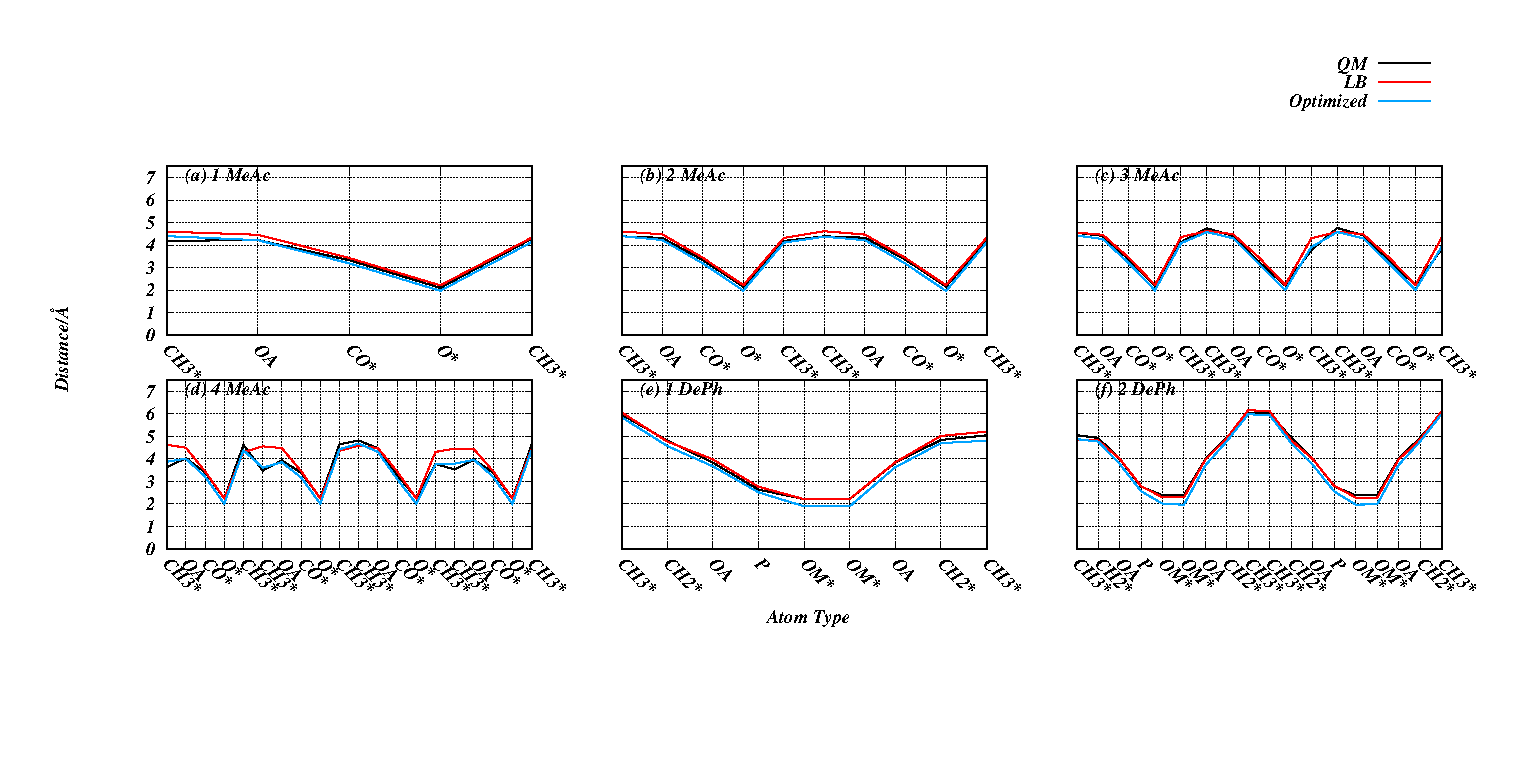
\includegraphics[width=0.8\textheight]{figure_s1.eps}
\end{sidewaysfigure}
\clearpage
\begin{table}
    \caption{Nelder--Meade constraints. These values were used to constrain the parameter search space during the NM--optimization.}
    \label{tab:constraints}
    {\tiny
    \begin{tabularx}{\textwidth}{X|X|X|X|X|X|X|X|X|X|}
	        &\tbxmulticol{2}{X|}{NA-CH3}&\tbxmulticol{2}{X|}{NA-CH2}&\tbxmulticol{2}{X|}{NA-CO*}&\tbxmulticol{2}{X|}{NA-OA,-OM*,-O*,-P}&Additional Constraints\\\hline
		&Min&Max&Min&Max&Min&Max&Min&Max&N/A\\\hline
	\sigmaij (nm)&0.2&0.5&0.2&0.5&0.2&0.5&0.2&0.5&$\sigma_{ij}^{\text{NA-OM*}}
        \leq \sigma_{ij}^{\text{NA-P}}$ \\\hline
	\epsilonij (kJ/mol) &0&0.79&0&0.81&0&0.83&0.05&7&N/A\\\hline
    \end{tabularx}
    }
\end{table}
\clearpage
\begin{figure}[htb]
    \caption{ Lipid chain deuterium order parameters. $S_{CD}$s are computed for each carbon
        for the chains Sn1 (a) and Sn2 (b), starting at the second carbon in the chain. We see that the optmized system is still showing significant ordering in the lipid
    chains as a result of ion binding; however, the ordering is less pronounced than in the system simulated with LB rules, 
    and is closer to that of the simulation without salt. This
result corresponds with the smaller bilayer thickness in the optimized system.
}
    \label{fig:op}
    %\includegraphics[width=\textwidth,trim=-3cm 0 0 0]{chainorder.eps}
%    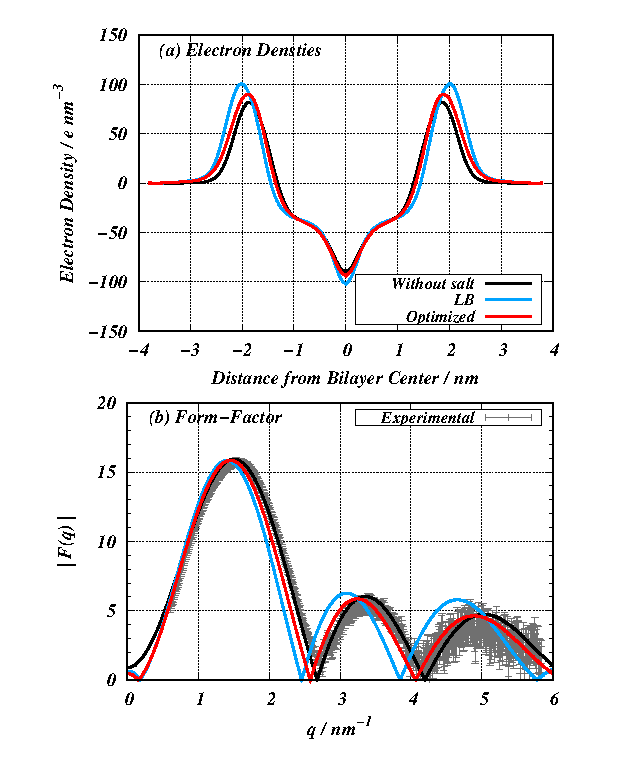
\includegraphics[width=\textwidth,trim=-3cm 0 0 0]{figure_4.eps}
    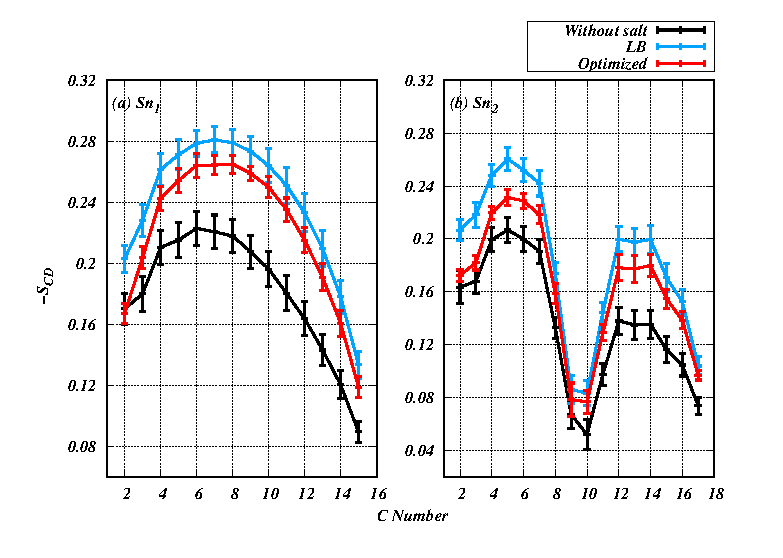
\includegraphics[width=\textwidth,trim=-3cm 0 0 0]{figure_s2.eps}
\end{figure}
\clearpage
\begin{figure}
    \caption{ Electrostatic potential as a function of distance from bilayer center. The optimized
cross terms yield a small change in the location of the peak of the potential in the
bilayer simulated with optimized cross terms, as well as the loss of the valley behind the peak.
}
    \label{fig:potential}
    %\includegraphics[width=\textwidth,trim=-3cm 0 0 0]{potential.eps}
    %\includegraphics[width=\textwidth,trim=-3cm 0 0 0]{figure_9.eps}
    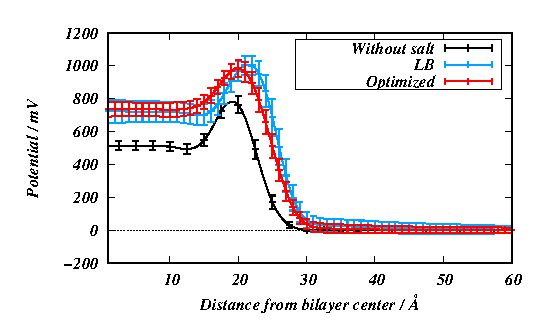
\includegraphics[width=\textwidth,trim=-3cm 0 0 0]{figure_s3.eps}
\end{figure}
\clearpage
\begin{figure}
    \caption{ Poisson-Boltzmann theory predictions and simulation results. (a) shows a snapshot of the 
system simulated with optimized cross terms, translated
to center the solvent occupied region. Water has been hidden
for clarity. (b) and (d)
    show the number density of ions in the solvent occupied region of the box. 
    (c) and (e) show the corresponding electrostatic potential in solvent.
    We illustrate theoretical predictions as solid lines, with corresponding 
    simulation results as points with error bars. Red vertical lines denote the \emph{hydration boundary} of the lipid bilayer. 
    \cl density data is used for fitting in both systems. 
}
    \label{fig:gouy}
    %\includegraphics[width=\textwidth,trim=0 0 0 0]{gouy.eps}
    %\includegraphics[width=\textwidth,trim=0 0 0 0]{figure_10.eps}
    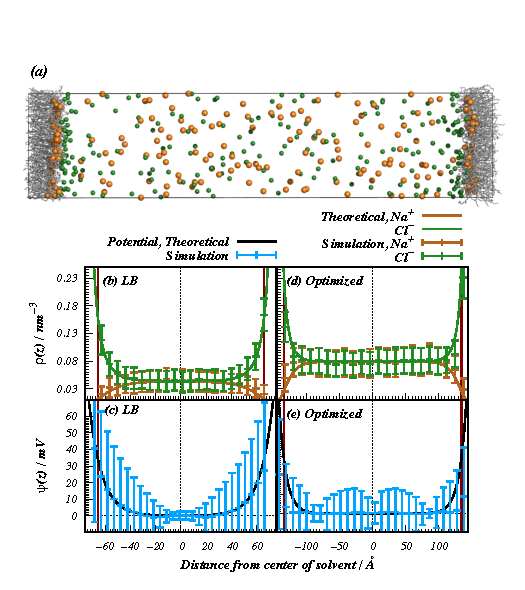
\includegraphics[width=\textwidth,trim=0 0 0 0]{figure_s4.eps}
\end{figure}

\end{document}
